\input{/Users/daniel/github/config/luapre.sty}%This is available at github.com/danimalabares/config
\input{/Users/daniel/github/config/thms-eng.sty}%This is available at github.com/danimalabares/config

%\usepackage[utf8]{inputenc}
%\usepackage[T2A]{fontenc}
%\usepackage[style=alpha,backend=bibtex]{biblatex}
%\addbibresource{bibliography.bib}

\begin{document}
\bibliographystyle{alpha}

\begin{minipage}{\textwidth}
	\begin{minipage}{1\textwidth}
		Advisor: Sergey Galkin \hfill Daniel González Casanova Azuela
		
	{\small\href{https://github.com/sergunchik/daniel}{github.com/sergunkchik/daniel}\hfill\href{https://github.com/danimalabares}{github.com/danimalabares}}
	\end{minipage}
\end{minipage}\vspace{.2cm}\hrule

\vspace{10pt}
{\huge Research journal}

A place to keep track of what I read. Colors don't mean anything in particular.

\tableofcontents

\section{Calabi-Yau threefold of degree 20 in $\mathbb{P}^7$}

\begin{thing4}{Research problem}[Telegram message from Sergey]\leavevmode
	Show or disprove the existence of a Calabi-Yau threefold of degree 20 in $\mathbb{P}^7$ that degenerates to Stanley-Reisner scheme of Gr\"unmbaum's triangulated 3-sphere with 8 vertices.

	Maybe predict some more elaborate invariants of this CY3, if it exists (in principle, there could also be more than one different smoothing).

	Grzegorz Kaputska told me the deformation space is described, but I do not remember the answer.

One way to attack the problem: look for the pool of constructions of codimension 4 varieties, and try to find something in this pool.
\end{thing4}

\subsection{Overview of this project in a Telegram message}

\begin{thing7}{Telegram message}[October 16]\leavevmode
	Recall that the objective of this project is to find a CY3 associated to a specific simplicial complex $\mathcal{M}$ called \textit{\textbf{Grünbraum sphere}}. This simplicial complex has 8 vertices, 20 facets, is homeomorphic to the 3-sphere but it is not the boundary of any 4-polytope.

	There is a scheme called \textit{\textbf{Stanley-Reisner scheme}} associated to any simplicial complex. To construct it, map the vertices of the simplicial complex to indeterminantes of a polynomial ring, compute a certain ideal and then take Proj. I have computed a Gröbner basis for the ideal corresponding to $\mathcal{M}$. Here's the result from GAP:
 
\texttt{gb:=[r.6*r.7*r.8, r.4*r.6*r.8, r.3*r.7*r.8, r.3*r.5*r.7, r.3*r.4*r.8, r.2*r.7*r.8, r.2*r.5*r.7, r.2*r.5*r.6, 
r.2*r.4*r.7, r.2*r.4*r.6, r.1*r.4*r.6, r.1*r.4*r.5, r.1*r.3*r.8, r.1*r.3*r.6, r.1*r.3*r.5, r.1*r.2*r.5];}

where every \texttt{r.i}  corresponds to one of the 8 vertices of the Grünbraum sphere as well as an indeterminante in the polynomial ring $k[$\texttt{r.1},…,\texttt{r.8}$]$.

 A smoothing of the resulting scheme (Proj of the ideal generated by those monomials) should be a CY3, so for the last weeks I've been trying to figure out how to figure out whether the smoothing exists or not.

 Here are some papers I’ve used:

 1. The paper by \cite{grun} (posted above in this chat) where they find $\mathcal{M}$ and claim to enumerate all the different combinatorial types of 4-dimensional simplicial convex polytopes with 8 vertices. Here I found the combinatorial data of M.

 2. \cite{luk1} where he shows that Grünbraum and Sreedharan made a mistake in their classification. Mimicking his computations I found the gröbner basis for the SR ideal of $\mathcal{M}$ above.

 3. \cite{jan1}. Here is a worked example on how to deform the SR scheme of a 7-vertex equivelar triangulation of the torus: "Here the toric geometry of $\operatorname{Def}^a_{X}$ [deformation functor] is extremely nice and and leads to a CY3 with Euler number 6".

 4. \cite{jan2}. A general description of how is the deformation space of SR schemes. This paper is strongly based in another by the same two authors, \cite{jan3}. Indeed: it looks like the main tool for describing the deformation space is cotangent cohomology. The latter paper gives a description of these cohomology modules. Can anyone tell if studying these cotangent cohomology theory is a good way to go?


 Finally, it was suggested by Sergey to use Pfaffian varieties as an example “to apply the machinery of tropical and SR things”—“tropical varieties are related to deformations/degenerations of everything”. Put some exercise about this in GAV course? Some of you are already familiar with Pfaffian varieties?
\end{thing7}

\subsection{Reading \cite{luk1}}

{\color{1}I had some earlier notes on this paper but I'll put here a summary dating September 6:}
\vspace{1em}

Let's do an overview of this project:

\begin{itemize}
	\item It all starts with \cite{grun} in 1967 saying they have classified all the different combinatorial types of 4-dimensional simplicial convex polytopes with 8 vertices. There is a peculiar one called $\mathcal{M}$.

	\item At some point \cite{luk1} noticed there were some mistakes in this classification using the main theorem in \cite{luk1}:

		\begin{thing2}{Theorem 0.1}\leavevmode
			Let $\Delta$ be a 4-simplicial polytope with $n+1$ vertices. Then the projective Stanley-Reisner scheme $\mathbb{P}(\mathcal{K}_{\Delta})$ is Gorenstein and nondegenerate simply normal crossing pseudo Calabi-Yau threefold. If we assume that there is a smoothing family $\mathcal{X}$ such that the central fiber $\mathcal{X}_0=\mathbb{P}(\mathcal{K}_{\Delta})$ then a general fiber $\mathcal{X}_t$ is also Gorenstein nondegenerate pseudo Calabi-Yau threefold and the degree of $\mathcal{X}_t$ satisfy the lower and upper bound.
		\end{thing2}
		{\color{9}In case you don't know what is going on here are some definitions:}

		Let $[n]$ be the set of all positive integers from 0 to $n$, and let $\Delta_n$ denote the power set of $[n]$. A subset $K\subseteq \Delta_n$ we call \textit{\textbf{simplicial complex}} if for every $f\in K$ all the subsets of $f$ are also in $K$. Let $P=k[x_0,\ldots,x_n]$ be a polynomial ring in $n+1$ variables over an algebraically closed field $k$. If $a=\{i_1,\ldots,i_k\} \in\Delta_n$ then we write $x_a\in P$ for the square free monomial $x_{i_1}\cdot \ldots\cdot x_{i_k}$. A simplicial complex $\mathcal{K}\subset \Delta_n$ gives rise to the ideal
		\[I_{\mathcal{K}}:=\left<x_a: a\in\Delta_n\setminus \mathcal{K}\right> \subseteq P\]
		{\color{persimmon}that is, the \textit{\textbf{Stanley-Reisner ideal}} is generated by the monomials that that are \textit{not} in the polytope.}

		The \textit{\textbf{Stanley-Reisner ring}} is $A_{\mathcal{K}}:=P/I_{\mathcal{K}}$. We associate an affine scheme $\mathbb{A}(\mathcal{K}) =\operatorname{Spec}(A_{\mathcal{K}})$ and projective scheme $\mathbb{P}(\mathcal{K})=\operatorname{Proj}(A_{\mathcal{K}})$.
		
		So he shows Gr\"unbraum and Sreedharan wrong using that
		
\begin{thing5}{Proposition 3.2}\leavevmode
			Let $\Delta$ be a $d$-simplicial polytope and let $X=\mathbb{P}(\mathcal{K}_{\Delta}$ be projective Stanley-Reisner scheme. Then $X$ is Gorenstein if and only if $\dim_k\tilde{H}_{d-1}(\Delta)=1$. In particular if $d>1$ then $X$ is Gorenstein iff $\dim_kH_{d-1}(\Delta)=1$.
\end{thing5}
		And them
\begin{thing5}{Proposition 3.3}\leavevmode
			For the examples one, seven and twenty-nine of 4-simplicial polytopes from the Table 4 in \cite{grun} the corresponding simply normal crossing pseudo Calabi-Yau threefolds cannot be Gorenstein.
\end{thing5}	
But to show (I think) that $\dim_kH_{d-1}(\Delta)\neq 1$ there is some minimal resolutions computed using \texttt{Macaulay2} software to show that
		\begin{quotation}
			each of the three exampls are not Gorenstein minimal free complex resolution because in the each case the last terms are of the rank five. This gives us the contradiction with the proposition 3.2.
		\end{quotation}
		
	\item And then what? Back to Telegram initial motivation message:

		\begin{quotation}
			Show or disprove existence of Calabi-Yau threefold of degree 20 in $\mathbb{P}^7$ that degenerates to Stanley-Reisner scheme of Gr\"unbraum's triangulates 3-sphere with 8 vertices.

			Maybe predict some more elaborate invariants of this CY3, if it exists (in principle, there could also be more than one different smoothing).

			Grzegorz Kapustka told me the deformation space is described, but I do not remember the answer.

			One way to attack the problem: look for the pool of constructions of codimension 4 varieties, and try to find something in this pool.
		\end{quotation}

		\item This leads to the desire of understanding deformation spaces using  \cite{jan1}. I read this over the summer (winter?) holidays and learnt some basic notions of deformation spaces. {\color{magenta}Next objective: wrap up what was learnt in \cite{jan1} and prepare to try to understand the deformation space.}
		
\end{itemize}

\subsection{Reading \cite{sturm}}

Here's some notes on \cite{sturm}, sec. 9.2, from sometime around June.
\vspace{1em}

{\color{orange}Looks like it would be nice to understand how minors are related to CYs}

\begin{exercise}[Sturmfel, 9.5.3]
	Let $I$  be the ideal of $3\times 3$-minors of a $3\times 4$-matrix of indeterminates. Compute the Bergman complex $\mathcal{B}(I)$ of this ideal.
\end{exercise}

\begin{defn}[Bergman complex and Bergman fan]
	Given any variety $X$  in $(\mathbb{C}^*)^n$  we define the \textit{\textbf{Bergman complex}} $\mathcal{B}(X)$  of the unit $(n-1)$-sphere $S^{n-1}$  in $\mathbb{R}^n$  as follows. A point $p \in S^{n-1}$ lies in $\mathcal{B}(X)$ is and only if there exists a sequence of vectors $p^{(1)},p^{(2)},p^{(3)},\ldots$ in $\mathbb{R}^n$ such that
\begin{equation*}
	p^{(r)}\in \log(X)\cap r\cdot S^{n-1}\text{ for all } r\geq 1\quad\text{ and}\quad \lim_{r \to \infty} \frac{1}{r} \cdot p^{(r)}=p	
\end{equation*}
	And the \textit{\textbf{Bergman fan}} $\widetilde{\mathcal{B}}(X)$  is the subset of vectors in $\mathbb{R}^n$  such that either $p=0$  of $\frac{1}{\|p\|} \cdot p$  lies in $\mathcal{B}(X)$.
\end{defn}
So the point of this object is that
\begin{thm}[9.6, fan is union of cones and complex is polyhedral complex]
	The Bergman fan $\widetilde{\mathcal{B}}(X)$ of a $d$-dimensional irreducible subvariety $X$ of $(\mathbb{C}^*)^n$ is a finite union of rational $d$-dimensional convex polyhedral cones with apex at the origin. The intersection of any two cones is a common face of each. Hence $\mathcal{B}(X)$ is a pure $(d-1)$-dimensional polyhedral complex.
\end{thm}

\begin{thm}[9.12, complex of matroid is polyhedral complex]
	The Bergman \\complex $\mathcal{B}(M)$ of a rank $d$ matroid $M$ is a pure $(d-2)$-dimensional polyhedral complex embedded in the $(n-2)$-sphere.
\end{thm}

\begin{thm}[the fan is the tropical variety]
	Let $I$ be an ideal in $\mathbb{Q}[x_1,\ldots,x_n]$ and $X$ be the variety it defines in $(\mathbb{C}^*)^n$. Then the tropical variety $\operatorname{trop}(I)$ equals the Bergman fan $\mathcal{B}(X)$.
\end{thm}
In the more general case when $t$ does appear in $I$, the topical variety $\operatorname{trop}(I)$ is not a fan, but it is a polyhedral complex with possibly many bounded faces.

But also have a look at this:
\begin{defn}[initial form and initial ideal]
	For a fixed vector $\omega\in \mathbb{R}^{n}$ and any Laurent polynomial $f=\sum c_\alpha x^\alpha$, the \textit{\textbf{initial form}} $\operatorname{in}_\omega(I)$ is the sum of all terms $c_\alpha x^\alpha$ such that {\color{magenta}the inner product $\omega\alpha$ is maximal, (what?)}.

	The \textit{\textbf{initial ideal}} $\operatorname{in}_\omega(I)$ is the ideal generated by the initial forms $\operatorname{in}_\omega(f)$ where $f$ runs over  $I$.
\end{defn}

What is this any good for?
\begin{lemma}[description of Bergman fan in terms of initial ideals]
	Let $X$ be any variety in $(\mathbb{C}^*)^n$ and $I$ its vanishing ideal. Then
	\[
		\widetilde{\mathcal{B}}=\{\omega\in \mathbb{R}^{n}:\operatorname{in}_\omega(I)\text{ does not contain a monomial} \} 
	.\]
	
\end{lemma}

Let's try to do the exercise:
\begin{proof}[Solution]
	Whaaaat?	
\end{proof}

Let's try
\begin{exercise}[9.5.(1)]
	Draw the graph and variety of the tropical polynomial
	\[
	f(x)=10+2x+7x^2+4x^3+0x^4
	.\]
\end{exercise}

\subsection{Reading \cite{def0}}

{\color{2}Just to record that in June-July 2024 I went over the beginnings of \cite{def0}. I won't put the notes here since I haven't used them since.}

But let me put why I was motivated to read that:

\begin{thing14}{Sergey}[June 26]\leavevmode
	Stanley-Reisner scheme of any complex is never CY in strict sense - it is usually very non-smooth and reducible (non-irreeducible), unless it is a single projective space (which is not CY either, but log-CY). Nice CY in usual sense (smooth projective varieties with trivial $K_X$) sometimes can \textit{degenerate} into SR schemes. So we are looking for something not as bizarre as SR scheme itself, that degenerates into these SR schemes.
\end{thing14}

\subsection{Reading \cite{jan1}}

Here's a summary of this paper dating September 23:

 \begin{itemize}
\item In \cite{jan2} they had already studied the Stanley-Reisner schemes of triangulated manifolds with regular edge graphs. The formal versal deformation spaces are nicely presented, with: in fact binomials. These surfaces are either torus or Klein bottles, and  \cite{jan1} is about the torus case.

\item So the point is that the deformation space $\operatorname{Def}_{X}^a=\mathcal{O}_{(X, \mathcal{O}_X(1))}$ is defined by some binomials and this allows \cite{jan1} to use Eisenbud and Sturmfelds "to realize smoothing components as toric varieties".

\item The main computational part of the article is about the cones and lattices of these toric varieties. Then these results are applied to statements about deformations.

\item Interestingly, "There should be a connection between the results in this paper and the moduli of polarized abelian surfaces".

\item The last section deals in detail with the vertex minimal triangulation of the torus, sometimes called the Möbius torus, with 7 vertices. Here the toric geometry of $\operatorname{Def}_{X}^a$ is extremely nice and leads to a Calabi-Yau 3-fold with Euler number 6. 
\end{itemize}

Here's the only 7-vertex (equivelar) triangulation of the torus.

\begin{figure}[H]
	\centering
	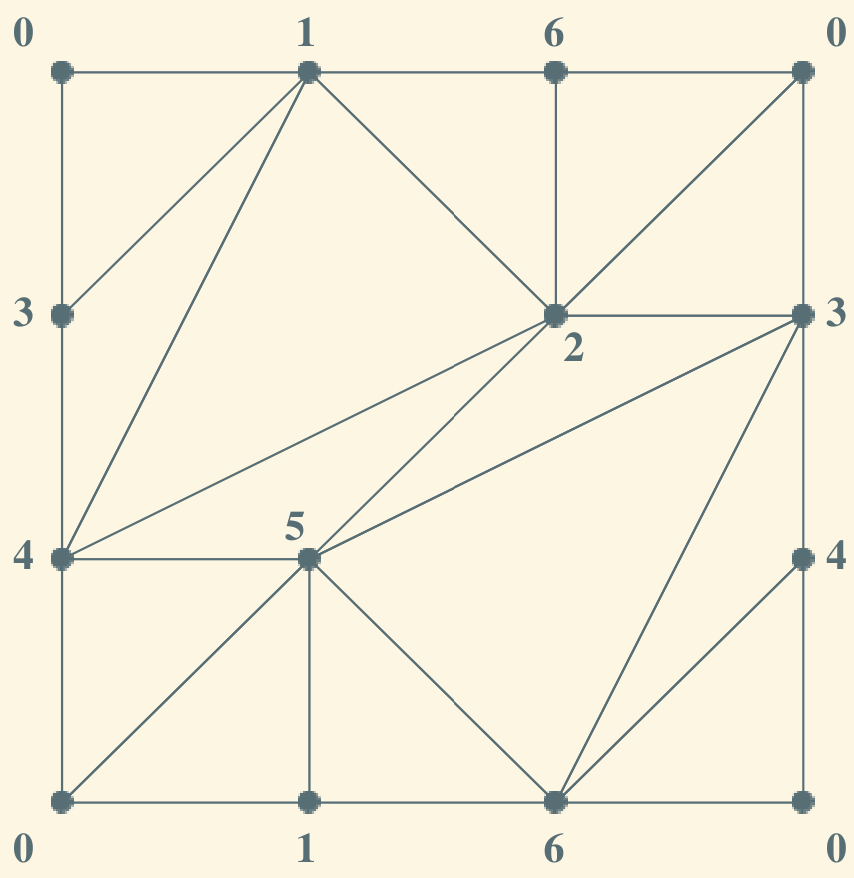
\includegraphics[width=0.3\textwidth]{fig1}
	\caption*{$T_7$}
\end{figure}

And I'm interested in seeing how come "the toric geometry of $\operatorname{Def}_{X}^a$ is extremely nice and leads to a Calabi-Yau 3-fold with Euler number 6".

\subsubsection{How \cite{jan1} gets a CY3}
\begin{enumerate}
\item \cite{jan1} gets a reflexive polytope $\Delta$.
\item The polytope determines a Fano variety $Y$.
\item The Minkowsky decomposition gives 3 divisors $E_i$ on $Y$.
\item Cut $Y$ with a general section of each of the $\mathcal{O}_Y(E_i)$.
\item The result is a Calabi-Yau 3-fold.
\item Take a crepant resolution and you get a Calabi-Yau 3-manifold.
\end{enumerate}

So it looks like here there is some toric geometry. Everything is very linked to the polytope $\Delta$: "More may be said about $\Delta$ but I have not been able to find a good description of it. Also the cones are very important.

So, before delving into toric geometry theory, next section goes back to the smoothings.

\subsubsection{January 22,26: construction of torus tiling, \(\operatorname{Def}_X^a\) is a vector space generated by the edges}
\textbf{Motivation}

In an attempt to bring my research more down-to-earth I will try to advance in the search for Grünbraum sphere smoothing. (Because this is an actual problem that could be solved.)

So I need to know how is the deformation space of the SR scheme associated to \(\mathcal{M}\) and \textit{find in there} a CY3.

Here's a quote from \cite{jan1}:
\begin{quotation}
	In \cite{jan2} we showed that triangualated surface manifolds with regular edge graph of degree 6 give SR schemes with nicely presented formal versal deformations spaces defined by polynomials, in fact binomials.
\end{quotation}
So initially \textbf{we don't know how combinatorially nice is \(\mathcal{M}\)}.

Anyway the important thing is that \cite{jan1} considers ``the versal formal element of [the functor] \(\operatorname{Def}_{X}^a\)"

Let me ask:
\begin{question}\leavevmode
	Are the smoothing components of \(\mathbb{P}(\mathcal{M})\) toric varieties?
\end{question}

\textbf{How \cite{jan1} does it} 

In an attempt to understand the combintorics of \(\mathcal{M}\) (and then its deformation space), let's have a look at the nice case in \cite{jan1}. It's a torus constructed as follows: consider the regular triangle tiling of the plane \(\{3,6\}\) and a ``sublattice [\(\Gamma\) ] of finite index" of the vertices. {\color{6}(I think of this sublattice as generated by any two linearly intependent vectors in \(\{3,6\}\).)}

\begin{figure}[H]
	\centering
	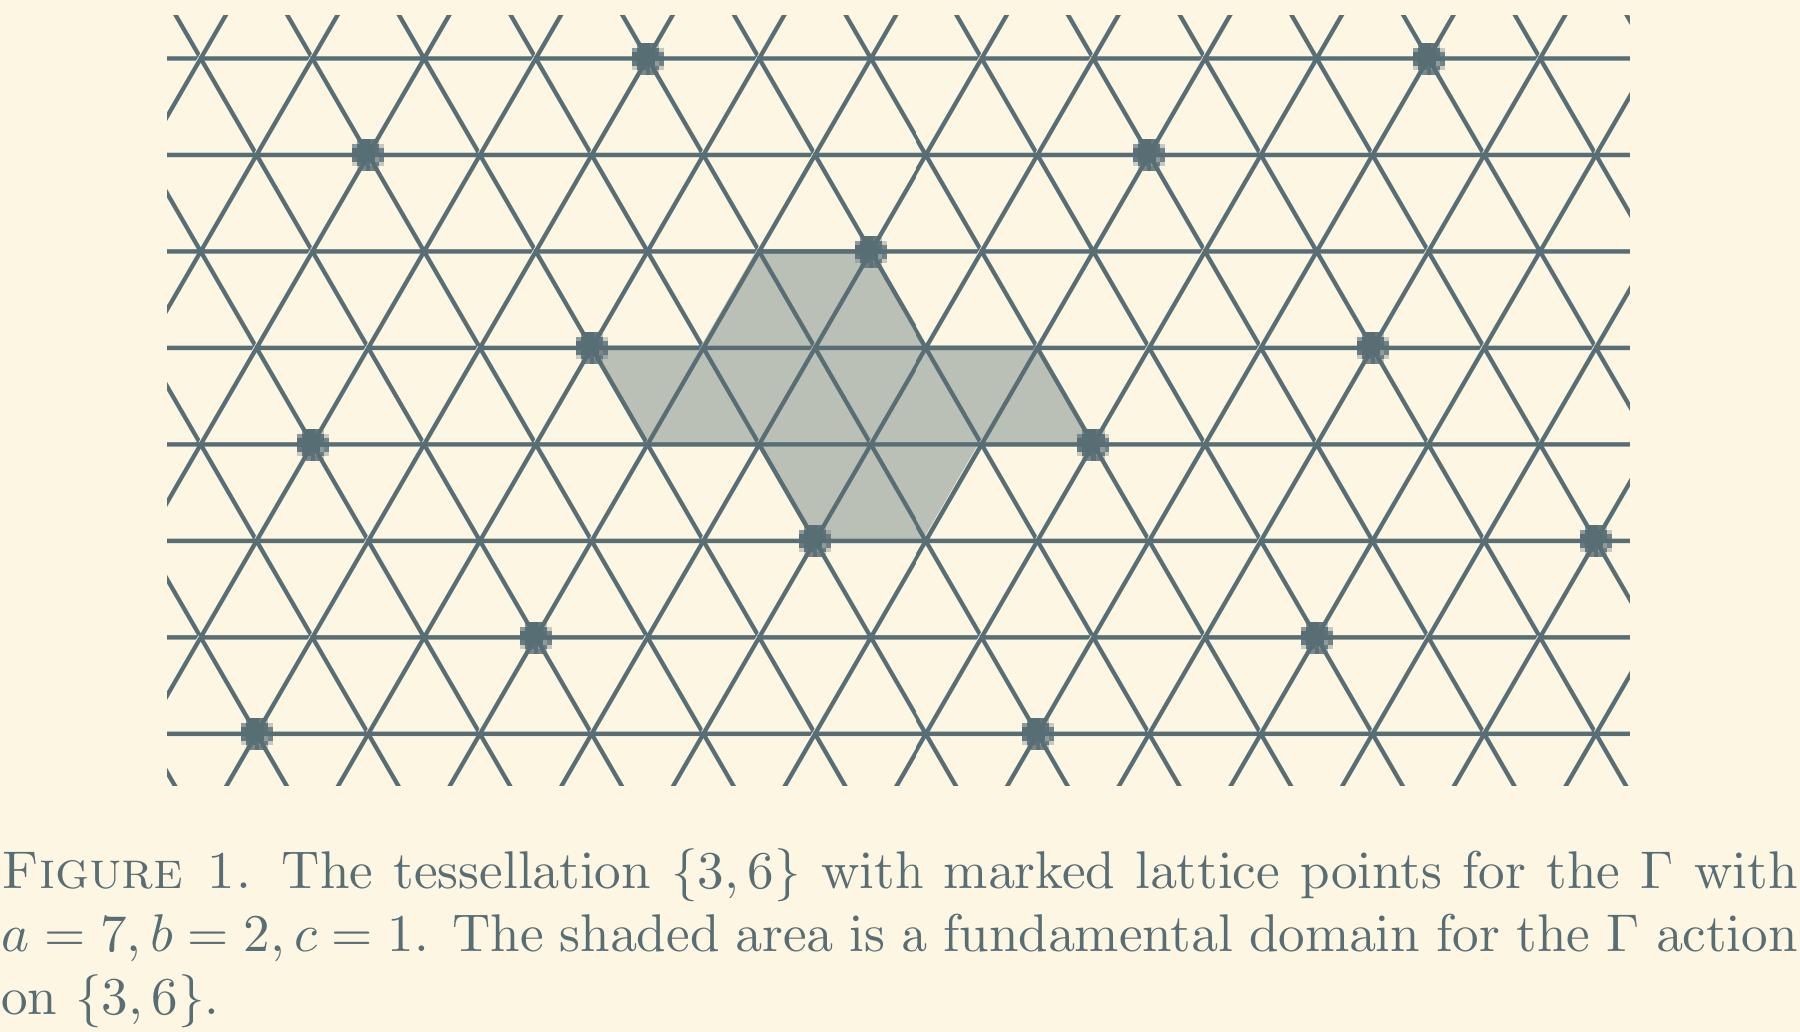
\includegraphics[width=0.9\textwidth]{fig3}
	\caption*{$T_7$}
\end{figure}
Taking the quotient \(\{3,6\}/\Gamma\) gives an equivelar (all vertices have the same valency and all faces have the same number of vertices) triangulation of the torus. {\color{6}I think this triangulation is just \(\{3,6\}\) on top of the quotient \(\mathbb{R}^2/\Gamma\cong \mathbb{T}^2\).}

Then, in Section 2 ``Overview" \cite{jan1} also defines \(G=\mathbb{T}/\Gamma\), which looks essentialy the same as \(T\), which is defined as \(T=\{3,6\}/\Gamma\), where \(\mathbb{T}\) is the lattice generated by \((1,0), \frac{1}{2}(1,\sqrt{3} \), so basically \(\{3,6\}\). The point is that \(T\) is the geometric object and \(G\) its automorphism group. Now the ``central observation […] allows us a natural identification of the elements of \(G\) and \(\operatorname{v ert}T\) […]", which is done via the Cayley graph: \textbf{Prop. 2.1} The edge graph of \(T\) is the Cayley graph of  \(G\). So, like in the olden days back in Mexico, the tiling is also the Cayley graph of its automorphism group.

Also \(\tau_k\) for \(k=1,2,3\) are the translations about the basic two vectors and what looks like the third edge on that triangle. Any pair of them generate the group. An edge in \(T\) is of \textit{\textbf{type \(k\)}} if it is of the form \(\{p,\tau_k(p)\}\).

Then the notation that once fixed \(k \in \{1,2,3\}\) then \(i,j\) are remaining two elements of \(\{1,2,3\}\setminus \{k\}\).

And then a big hint on what \(\operatorname{Def}_{X}^a\) is. First remember what Dani from the past once wrote:
\begin{quotation}
	``And remember that $\operatorname{Def}^a_{X}$ is the functor of Artin rings $\operatorname{Def}^a_{X}:\mathcal{A}\longrightarrow \operatorname{Sets}$ that maps an Artin ring, I guess, to the moduli space of deformations of $(X,\mathcal{O}_X(1))$over $A \Big/$isomorphism."
\end{quotation}
And guess what, \(\operatorname{Def}_{X}^a\) has a tangent space. And its tangent space has a basis \(\varphi_{p,q}\) for an edge \(\{p,q\}\in T\). In the \(ijk\) notation, the ``corresponding perturbation" ({\color{6}so maybe by ``perturbation" he means vector tangent to the deformation space, which makes sense intuitively}) this is
\[\varphi_{p,\tau_k(p)}(x_m)=\begin{cases}
\frac{x_m x_p x_{\tau_k(p)}}{x_{-\tau_i(p)}x_{-\tau_j(p)}}\qquad &\text{ if \(\{-\tau_i(p),-\tau_j(p)\} \subseteq m\)}  \\
	0\qquad &\text{otherwise.} 
\end{cases}\]
What is this thing? It's a function that takes polynomials and gives rational functions. How is this a tangent vector.

Again:

\begin{quotation}
	``If \(\mathcal{K}\) is a combintorial manifold without boundary then
	\[\operatorname{Def}_{\mathbb{P}(\mathcal{K})}^a(C[\varepsilon])\simeq H^{0}(\mathbb{P}(\mathcal{K}),\mathcal{T}^1_{A_{\mathcal{K}},0})\simeq T^1_{A_{\mathcal{K}},0}\]
\end{quotation}
So do have a look at that term in the middle: its the sections of the Proj of \(A_\mathcal{K}\) (the SR \textit{ideal} of the simplicial complex \(\mathcal{K}\)…), which probably is what we call ``combinatorial manifold", with respect to \(\mathcal{T}^1\) which is…

\begin{thing2}{Summary of January 27}\leavevmode
Looks like understanding why \(\operatorname{Def}^a_{\mathbb{P}(\mathcal{K})}\) is also the sections of a bundle could help me understand what it is. I want to know that \(\mathcal{T}\) is and its relationship with \(T^1_{A_{\mathcal{K}},0}\). The problem is that \cite{def0} extremely technical in defining the "cotangent modules". How to get around this? At least the simplicial complex \(\mathcal{K}\) is around in these equations, so maybe before too long I can put my combinatorial data from \(\mathcal{M}\).
\end{thing2}

\begin{thing5}{Note from January 29}\leavevmode
Looks like \(H^1\) is in correspondence with the set of deformations; if  \(H^1\) is trivial then the object is rigid. \(H^2\) is the obstructions: Thm 1.9 from Lucas: \(H^2\) is trivial then \(X\) is unobstructed.
\end{thing5}

[This was written before Jan 27] and in \cite{jan2} we see that
\begin{quotation}
	``for an \(S\)-algebra \(A\) and \(A\)-module \(M\) there exist the cotangent modules \(T^i_{A/S}(M)\). We write \(T^i_A\) when \(S=k\) and \(M=A\). The module \(T^0_A=\operatorname{Der}_k(A,A)\) consists of the infinitesimal automorphisms of \(A\), \(T^1_A \simeq \operatorname{Def}_{\operatorname{Spec}A}\) is the space of first order deformations of \(\operatorname{Spec}A\) and \(T^2_A\) contains the obstructions for lifting deformations."
\end{quotation}
\label{varphis}
And what's great is that (back to  \cite{jan1})
\begin{quotation}
	``It follows from the results in \cite{jan2} that if \( \mathcal{K}\) is a combinatorial manifold without boundary and all vertices have valency greater than or equal to 5, then \textbf{\(T^1_{A_\mathcal{K},0}\) is the $\mathbb{C}$-vector space on the edges of \(\mathcal{K}\)}. Since \(\mathcal{K}\) is a manifold, the link of an edge must be two vertices, […]. If \(\varphi_{p,q} \in T^1_{A_\mathcal{K},0}\) is the basis element corresponding to \(\{p,q\}\) and \(x_m\) is in the SR ideal, then 
\[\varphi_{p,q}(x_m)=\begin{cases}
	\frac{x_mx_px_q}{x_ix_j}\qquad &\text{if \(\{i,j\}\subseteq m\)}  \\
	0\qquad &\text{otherwise.} 
\end{cases}\]
There is a natural \((n-1)\)-dimensional torus action on \(\operatorname{Proj}A_\mathcal{K}\) […]" [Which induces an action on \(T^1_{A_{\mathcal{K}},0}\)…]
\end{quotation}
So,
\begin{quotation}
	{\color{6}to me it looks like \(\operatorname{Def}_X^a\) is a vector space.}
\end{quotation}

\textbf{Up next:} ``Let \(t_{p,q}\) be the dual basis of coordinate functions on \(\mathbb{C}^{3n}\)". {\color{4}What does that mean?} That is the first step towards using the theory of Sturmfelds, so 1 and a half pages of that. \textbf{For tomorrow:} keep trying to read \cite{jan1}. There is a lot of very dense things, but maybe skipping to Deformations section, looking at some examples. Recall that maybe it's possible to apply (at least the first steps) of this whole construction to the case of our simplicial complex \(\mathcal{M}\). So either keep reading \cite{jan1}, or try to apply what has been learnt to \(\mathcal{M}\)? Is it too soon?

\iffalse\begin{upshot}[Dani]\leavevmode
The Stanley-Reisner construction allows us to handle the simplicial complex algebraically (its faces are identified with monomials in the polynomial ring on the number of vertices). \textit{What is the SR scheme then?} Some geometric encarnation of the already geometric object that the simplicial complex is. And we want it smooth. 
\end{upshot}\fi

\begin{thing2}{A note from Pedro's seminar on deformation of algebras}\leavevmode
Equivalence of the derived categories of two objects gives an equivalence on their deformation spaces. Eles provaram uma equivalencia derivada. See \cite{pedro} more of Pedro's work.
\end{thing2}

\subsubsection{Computing the SR ideal of $\mathcal{M}$}

{\color{2}Just to record that around October 3 I went over the computation I had done in semester 2024.1 computing the SR ideal of $\mathcal{M}$. This motivated me to go over \cite{jan2}.} 

\begin{thing9}{Dani}[June 14]\leavevmode
	In Grünbaum and Sreedharan paper above it is shown that there are 37 combinatorial types of simplicial 4-polytopes with 8 vertices (thm 1). Combinatorial type refers to the incidence arangement of the faces (cells=facets, faces, edges and vertices). Simplicial means all the facets and hence all other faces are simplices.

	Theorem 2 in that paper shows the existence of a strange simplicial complex with 8 vertices and 20 facets, homeomorphic to the 3-sphere, that is not combinatorially equivalent to the boundary of any 4-polytope.
\end{thing9}

Luckily I had made some computations of this sort some time ago, which turned out good in the sense that… this is what happen(ed/will happen):

\begin{enumerate}
	\item In \texttt{python}: Define the polytope as a subset of the power set of $\{1,2,3,4,5,6,7,8\}=\Delta_8$. It is determined by a set of facets (subsets of $\Delta_8$ that I will find in \cite{grun}.

	\item In \texttt{python}: compute all the subsets of these facets (this is the complete polytope. Compute the complement of the poyltope with respect to  $ \Delta_8$.

	\item In \texttt{python}: tailor the output to give to \texttt{gfan} or \texttt{gap}.

	\item \texttt{gfan} or \texttt{gap} compute the grobner basis of the ideal. That's the SR ideal we are looking for. {\color{1}and now we have a gröbner basis if that matters.}
\end{enumerate}

\begin{thing3}{Dani}[October 5]\leavevmode
	Let's do this computation at once. Turns out I had already done that computation. Whoa! The Gröbner basis given by \texttt{GAP} is in \texttt{thinglc.g}:

{\color{4}\begin{quotation}
		\texttt {\#It is this one!}

	\texttt{gb:=[r.6*r.7*r.8, r.4*r.6*r.8, r.3*r.7*r.8, r.3*r.5*r.7, r.3*r.4*r.8, r.2*r.7*r.8, r.2*r.5*r.7, r.2*r.5*r.6, 
r.2*r.4*r.7, r.2*r.4*r.6, r.1*r.4*r.6, r.1*r.4*r.5, r.1*r.3*r.8, r.1*r.3*r.6, r.1*r.3*r.5, r.1*r.2*r.5];}
\end{quotation}}

$\mathsf{OK}$ so now I have a Gröbner basis for the Stanley-Raisner ideal $\mathcal{K}$ of my projective scheme. Now I want to compute the projective scheme itself, $\operatorname{Proj}(\mathcal{K})$. What is it or what's up? What are the singularities? What does it mean to smooth it? Theoretically it is the set of homogeneous prime ideals of $\mathcal{K}$

[…]

So I guess a natural question is \textbf{what is $\operatorname{Def}_{X}$?} I guess, for $X=\operatorname{Proj}(\mathcal{K})$.
\begin{thing3}{What happens now}\leavevmode
	is that I read more \cite{jan1} and \cite{jan2} and I understand how to deform Stanley-Reisner schemes.

	Here's a motivating quote for tomorrow:

{\color{7}\begin{quotation}
	Smoothings of Stanley-Reisner schemes associated to combinatorial manifolds yield interesting algebraic geometric varieties. For example if the complex is a triangulated sphere then the smoothing (if possible) would be Calabi-Yau. The Stanley-Reisner scheme of a triangulated torus would smooth to an abelian variety. A triangulated $\mathbb{R}P^{2}$ would give an Enriques surface. It is our hope that the results of this paper may be useful for the study of degenerations of such special varieties. 
\end{quotation}}
\end{thing3}

\end{thing3}

\subsection{Reading \cite{jan2}}

\begin{enumerate}
\item A little slow this morning but I reviewed the definition of scheme and its open sets (which was not quite necessary since we are dealing with $\operatorname{Proj}$… but $\mathsf{OK}$).
\item \cite{jan2} gives a list of combinatorial objects (the link, the open star, closed star, geometric realization, valency, …) associated to a simplicial complex. Then defines de Stanley-Reisner ring actually gives a description of the open sets of $\operatorname{Proj}(A_{\mathcal{K}})$ in terms of the link.
	\item Then there is a description of the cohomology using the irrelevant maximal ideal.

	\item In \textbf{section 2.3 The cotangent spaces and sheaves} there is an equation
		\[T_A^1=\operatorname{Def}_{\operatorname{Spec}(A)}(k[\epsilon])\]
		which is the \textit{\textbf{first order deformations}} of $\operatorname{Spec}(A)$. {\color{5}I'd like to understand this and find out if takes me any closer to understanding the deformation of my $\operatorname{Proj}(A_{\mathcal{K}_\mathcal{M}})$.}
\end{enumerate}

\begin{thing4}{Objective}\leavevmode
	Understand the deformation space of $\mathbb{P}(A_\mathcal{M})=\operatorname{Proj}(A_\mathcal{M})$ where $\mathcal{M}$ is Grünbraum sphere and $A_\mathcal{M}$ its associated Stanley-Reisner ring.
\end{thing4}

\begin{thing7}{Important remark}\leavevmode
\cite{jan1} obtains a CY3 from a nice triangulation of a torus. We are dealing with a crazy triangulation of a not-a-polytope simplicial complex called $\mathcal{M}$.
\end{thing7}

Ok so maybe some notes about what is the functor $\operatorname{Def}_{X}^a$? Well $a$ is for ample because "a projective SR scheme comes equipped with an very ample line bundle, so $\operatorname{Def}_{X}^a=\operatorname{Def}_{X,\mathcal{O}_X(1)}$.  \cite{jan1} will consider the versal formal element of this functor---versal comes from universal, some categorical property of the functor.

{\color{4}The trick in \cite{jan1} is that this functor $\operatorname{Def}_{X}^a$ is defined by binomial equations, so \cite{jan1} can use Sturmfels to "{\color{2}realize the smoothing components as toric varieries"}} And remember that $\operatorname{Def}^a_{X}$ is the functor of Artin rings $\operatorname{Def}^a_{X}:\mathcal{A}\longrightarrow \operatorname{Sets}$ that maps an Artin ring, I guess, to the moduli space of deformations of $(X,\mathcal{O}_X(1))$over $A \Big/$isomorphism.

{\color{8}$\mathsf{OK}$ so why is $\operatorname{Def}^a_{X}$ defined by binomials and how is $\operatorname{Def}^a_X$ defined for $\mathcal{M}$?}

$\mathsf{quickly!}$ because I'm almost out of time, but, it looks like a big part of the work done in \cite{jan2} actually comes from \cite{jan3}, a.k.a. \textit{Cotangent cohomology of Stanley-Reisner rings}. After several things, \cite{jan2} is "now able to describe $T^i_{\mathbb{P}(\mathcal{K})}$:

\begin{thing4}{Theorem 5.5}\leavevmode
	If $\mathcal{K}$ is a manifold then
	\begin{enumerate}[label=(\roman*)]
		\item $H^{0}(\mathbb{P}(\mathcal{K}),\mathcal{T}^1_{\mathbb{P}(\mathcal{K})})\cong \mathcal{T}^1_{A_{\mathcal{K},0}}$.
		\item $H^{1}(\mathbb{P}(\mathcal{K}),\mathcal{T}^1_{\mathbb{P}(\mathcal{K})})=0$.
		\item There are exact sequences
			\[\begin{tikzcd}
				0\arrow[r]&..\arrow[r]&..\arrow[r]&..\arrow[r]&0
			\end{tikzcd}\]
	\end{enumerate}
\end{thing4}

\begin{thing3}{Theorem 5.6}\leavevmode
	(dimension of $T^1_{\mathbb{P}(\mathcal{K})}$.
\end{thing3}

Now have a look at section 6. \textbf{Algebraic and non-algebraic deformations of $\mathbb{P}(\mathcal{K})$}.

{\color{4}\begin{quotation}
		We consider now the functor $\operatorname{Def}^a_{\mathbb{P}(\mathcal{K})}:=\operatorname{Def}_{(\mathbb{P}(\mathcal{K}),L)}$, $L=\mathcal{O}_{\mathbb{P}(\mathcal{K})}(1)$, of algebraic deformations.
\end{quotation}}

\begin{thing2}{Theorem 6.1}\leavevmode 
	If $\mathcal{K}$ is a manifold then … Thus
\[\operatorname{Def}^a_{\mathbb{P}(\mathcal{K})}(k[\epsilon ])\cong H^{0}(\mathbb{P}(\mathcal{K}),\mathcal{T}^1_{\mathbb{P}(\mathcal{K})})\cong T^1_{A_{\mathcal{K}},0}\]
and $H^{0}(\mathbb{P}(\mathcal{K}), \mathcal{T}^2_{\mathbb{P}(\mathcal{K})}) $ contains all obstructions for $\operatorname{Def}^a_{\mathbb{P}(\mathcal{K})}$.
\end{thing2}

{\color{8}\bfseries So he is describing $\operatorname{Def}^a_X$.}\hspace{.5em}

\subsection{Computing \(\operatorname{Def}^a_X\mathcal{M}\)}

The objective os this section is to compute the deformation space of \(\mathcal{M}\). First we must go over a little theory.

\subsubsection{Lucas' Notes on defos}

Once upon a time Lucas shared with us his notes on deformations. The file \texttt{lucas-defos.pdf} is now at \texttt{sergunchik/daniel/other-docs/}.

\begin{example}\leavevmode
``Taking closed points" (what could this mean?) we consider the quadric \(X=V(xy-t) \subseteq \mathbb{A}^3\) and the deformation
\[\begin{tikzcd}
	X \arrow[r,hook ]\arrow[dr,"\pi"]&\mathbb{A}^3\arrow[d]& (x,y,t)\arrow[d,maps to ]\\
	&\mathbb{A}^1&t
\end{tikzcd}\]
This is a quadraic:
\begin{figure}[H]
	\centering
	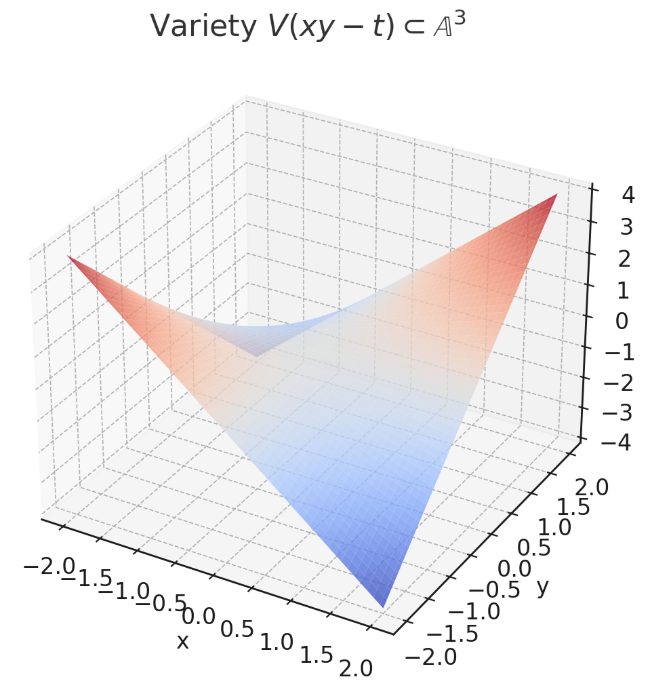
\includegraphics[width=0.5\textwidth]{fig4}
\end{figure}
But at \(t=0\) we get a singular fiber: it's the two axes. The rest of the deformations are smooth surfaces like the one on the picture.
\end{example} 

The reason why I'm feeling motivated to ``compute the deformation space of \(\mathcal{M}\)" is basically the discovery of

\begin{thing4}{Proposition 1.2.9}[\cite{def0}, \texttt{lucas-defos.pdf}]\label{prop:1.2.9}\leavevmode
Let \(X\) be an algebraic variety. There is a 1-1 correspondence
\[\kappa: \left\{ \substack{\text{isomorphism class of first order}  \\ \text{locally trivial deformations of \(X\)} } \right\} \longrightarrow H^{1}(X,T_X)\]
called the \textit{\textbf{Kodaira-Spencer correspondence}}, where \(T_X=\operatorname{Hom}(\Omega^1_X,\mathcal{O}_X)= \operatorname{Der}_k(\mathcal{O}_X,\mathcal{O}_X)\), such that \(\kappa(\xi)=0\) if and only if \(\xi\) is the trivial deformation class.

In particular if \(X\) is nonsingular then {\color{2}(but most likely \(\mathbb{P}(\mathcal{M})\) is highly singular)} you can remove the "locally trivial", ie.e. there is a bijection between isomorphism classes of first order deformations of \(X\) and \(H^{1}(X,TX)\).
\end{thing4}

\iffalse

\begin{thing2}{Big understanding}\leavevmode
Despite \(T_X\) looking like a tangent bundle, it is a cotangent bundle: \(T_X=\operatorname{Hom}(\Omega^1_X,\mathcal{O}_X)\).
\end{thing2}

So probably it is the \textit{\textbf{first cotangent module}} of \(R\) over \(A\) for some ring \(R\) and some algebra \(A\), denoted by \(T^1_{R/A}\). So the reason why that remained a mystery is that the formal (algebraic, \cite{def0}) definition of this object is as \(\operatorname{Ex}_A(R,R)\). (As confirmed in \href{https://seminarios.impa.br/visualizar/10126}{Pedro's talk yesterday} on deformation of algebras, there are lots of \(\operatorname{Ex t}\)s in this.)

Anyways according to Lucas' notes, for the proof of Kodaira-Spencer correpondence we'd have to use derivations. Moving on.

Then I'd have to read a bit on what obstructions are, and finally follow Lucas for an isomorphism \(\operatorname{Def}_X(D) \cong \operatorname{Ex t}^1_{\mathcal{O}_X}(\Omega^1_{\mathcal{O}_X}(\Omega^1_X,\mathcal{O}_X)\) and an exact sequence 
\[\begin{tikzcd}[column sep=small]
	0\arrow[r]&H^{1}(X,TX)\arrow[r]&\operatorname{Ex t}^1_{\mathcal{O}_X}(\Omega^1_X,\mathcal{O}_X\arrow[r]&H^{0}(X, \mathcal{E}\operatorname{x t}^1_{\mathcal{O}_X},\mathcal{O}_X)\arrow[r]&H^{2}(X,TX)
\end{tikzcd}\]

But maybe the true point in all this is that \textbf{I should compute \(H^{1}(X,TX)\) for \(\mathcal{M}\)}. 
\fi

\subsubsection{February 10}
Summary of today:
\begin{enumerate}
	\item I realised that the cohomology \(H^{1}(X,TX)\) in Kodaira-Spencer correspondence is the cohomology w.r.t. tangent bundle as defined in Lucas' notes using the ring \(\mathbb{C}[\varepsilon]=\mathbb{C}[x]/(x^2)\). Which means: \textbf{computing the space of locally trivial infinitesimal deformations of a SR scheme is computing this cohomology}.
	\item In \cite{jan1} it is claimed that if \(\mathcal{K}\) is any combinatorial manifold without boundary and all vertices have valency greater than or equal 5, then \(T^1_{A_\mathcal{K},0}\) is the \(\mathbb{C}\)-vector space on the edges of \(\mathcal{K}\).
	\item  \textbf{Next step}: make sure whether I am in the situation of the previous item.
\end{enumerate}

Looking into Lucas' notes, I realisa that actually \(TX\) \textit{is} the tangent bundle (defined in a certain algebraic way that matches the pointwise definition that \(T_pX=\left(\mathfrak{m}/\mathfrak{m}^2\right) ^*\). So it's literally computing the first cohomology group  of \(H^{1}(M,TX)\).

\subsubsection{February 11}

\begin{enumerate}
\item I reviewed my own notes: I realise that I have read the same passage on Kodaira-Spencer correspondence and the ``explanation of what \(\operatorname{Def}^a_X\) is" several times already. And I conclude that if \(\mathcal{M}\) is a combinatorial manifold (probably yes) then I already know the space of locally trivial deformations.
\item And what would I do next? I read \cite{jan1} again, and I discover that the \(\varphi\)'s, which I \hyperref[varphis]{had already studied}, will provide a base of the cotangent space.

	And that's already a big difference from our case, because the automorphism group of \(\mathcal{M}\) is probably very different from a torus: probably there are no translations!
\item Then  \cite{jan1} defines an ideal using the \(\varphi\)'s, and claims that ``The ideal \(I\) defines a versal base space in \((\mathbb{C}^{3n},0)\)" for \( \operatorname{Def}^a_X\). Then he proceeds (and we're still in the Overview section!) to do the Sturmfeld's thing, which is technical.
\item Next section description of the SR ideal (I have done this already) and then next section is called 4. Analysis. We have: a bunch of things related to the translations (4.1). 4.2 is Sat L so probably more Sturmfelds (or better yet, the part where he actually does the Sturmeflds part, not just overview). Last thing in this subsection is that the number of main components of \(\operatorname{Def}^a_X\) has been found.
\item  Then there is a subsection on some quotient \(M/ M'\) that I don't remember what it is, and then section 5. Deformations, which is where the smoothings are described.
\item So maybe: read some more about \(M/M'\), or… try to understand at once the combinatorial structure of \(\mathcal{M}\) and see how far you can go with it.
\end{enumerate}

\subsection{February 24: reading \cite{grun}}

I have been trying to understand the construction of \(\mathcal{M}\) from \cite{grun}. The main idea is to construct 4-polytopes with 8 vertices (the \(P^8\)'s) from 4-polytopes with 7 vertices (the \(P^7\)'s). Looks like this makes sense since the \(P^7\)'s appear to be classified in Table 1: theres five of them, \(P_1^7\) to \(P_5^7\), that have 11, 12, 13, 14 and 15 facets respectively.

So the method is to pick one of the \(P^7\)'s, call it \(Q\), and a point that is not in the affine span of any of the facets, and take the convex hull \(P\) of the whole thing. There is a simple definition to make sure this process is done correctly: a point is said to be \textit{\textbf{beyond}} a hyperplane not intersecting \(\int Q\), say \(H\), if it is in the half space determined by \(H\) that does not intersect \(Q\). The idea is to consider \(H\) to be the affine space determined by a facet of \(Q\).

Here's an idea I'm trying to grasp better:
\begin{quotation}
	Therefore the combinatorial structure of \(P\) is completely determined by the combinatorial type of \(Q\) and the \((d-1)\)-complex \(\mathcal{C}\) consisting of those facets of \(Q\) beyond which \(V\) is is, and their faces.
\end{quotation}
The thing is that it appears to me that there should only be one such facet (i.e. that \(\mathcal{C}\) should be a single facet).

Anyway, have a look at this quote in page 445 (this is a few pages ahead of the above quote):
\begin{quotation}
	However, with a given \(P^7\) and a complex \(\mathcal{C}\) on its boundary there is , in pcinciple, no guarantee for the existence of a point \(8\) that is beyond precisely those facets of \(P^7\) whih are in \(\mathcal{C}\). For a given combinatorial type of \(P^7\), and fixed \(\mathcal{C}\) on its boundary, such a point \( 8\) may exist, or fail to exist, depending on the particular polytope of type \(P^7\) chosen. Hence, strictly speaking, what we have constructed so far are not 4-polytopes with 8 vertices but certain combinatorial schemes, or 3-complexes, which may, or may not, be the boundary complexes of 4-polytopes.
\end{quotation}
Actually that looks great--it may be the beginnings of understand what was meant all along with that claim that \(\mathcal{M}\) is ``not the boundary of any  4-polytope".

\subsection{March 10: understanding \(\mathcal{M}\)}

Let's understand the construction of \(\mathcal{M}\). We start with a \(P^7\), i.e. a 4-polytope with 7 vertices, called \(Q\), and consider a vertex \(V\) that does not intersect \(Q\) nor any of the hyperplanes determined by the facets of \(Q\). Call \(P:=Q \cup  \{V\}\).
\begin{figure}[H]
	\centering
	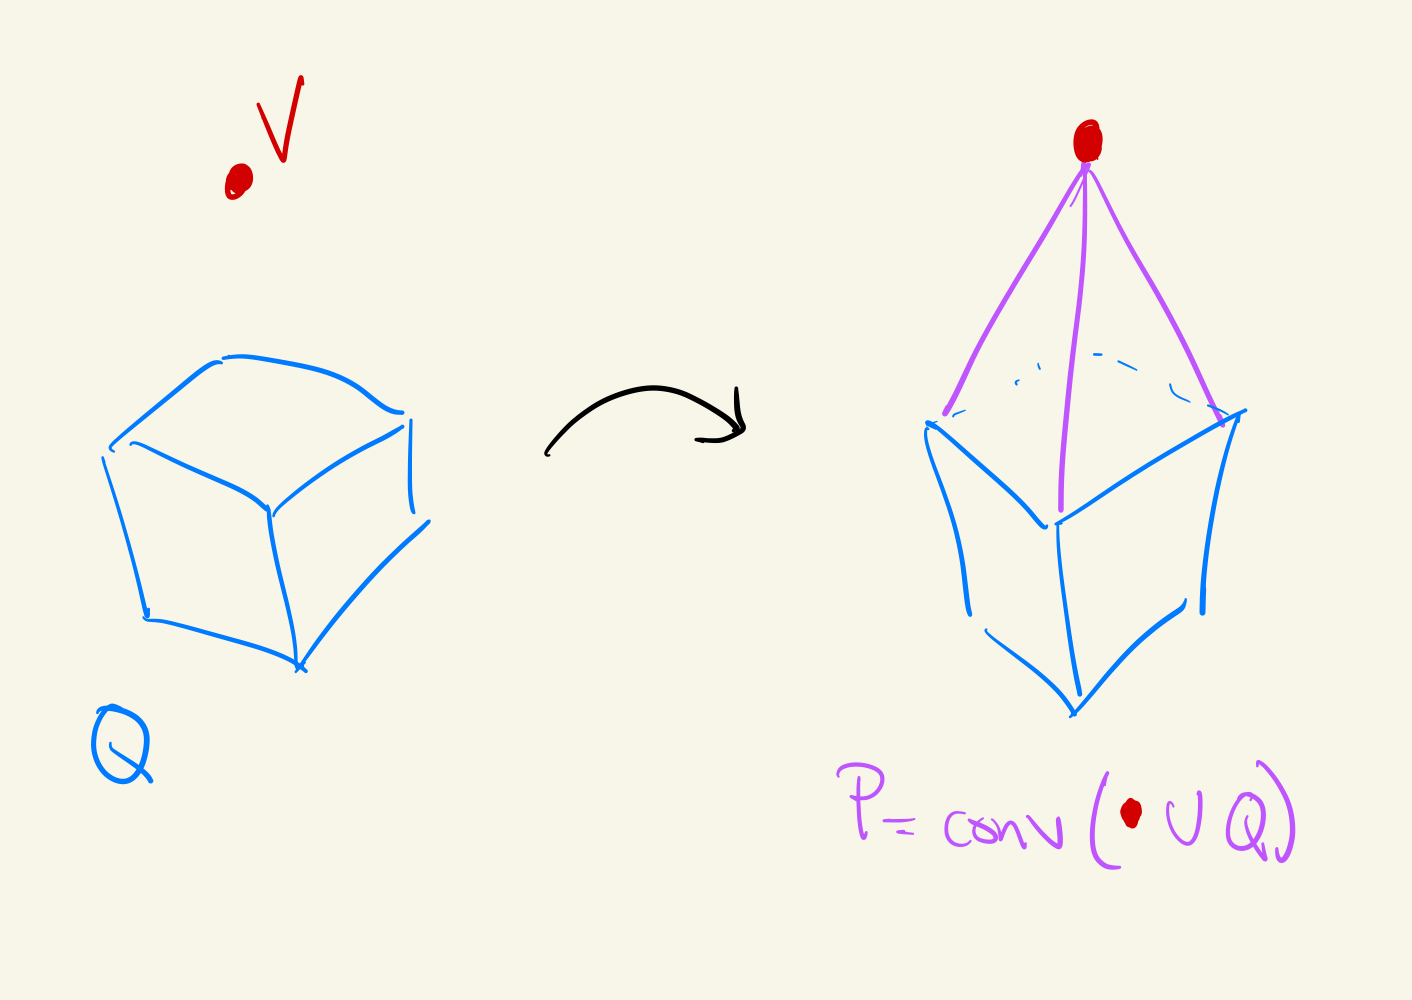
\includegraphics[width=0.5\textwidth]{fig5}
	\caption*{Construction of \(P\)}
\end{figure}
Then
\begin{quotation}
The facets of  \(P\) which do not contain \(V\) are precisely the facets of \(Q\) beneath which \(V\) is. The facets of \(P\) which contain \(V\) are precisely the sets of the form \(\operatorname{conv}(\{V\}\cup G)\) where \(G\) is a \((d-2)\)-face of \(Q\) such that \(V\) is beneath one of the facets of \(Q\) containing \(G\), and beyond the other such facet.
\end{quotation}

 \begin{figure}[H]
 	\centering
 	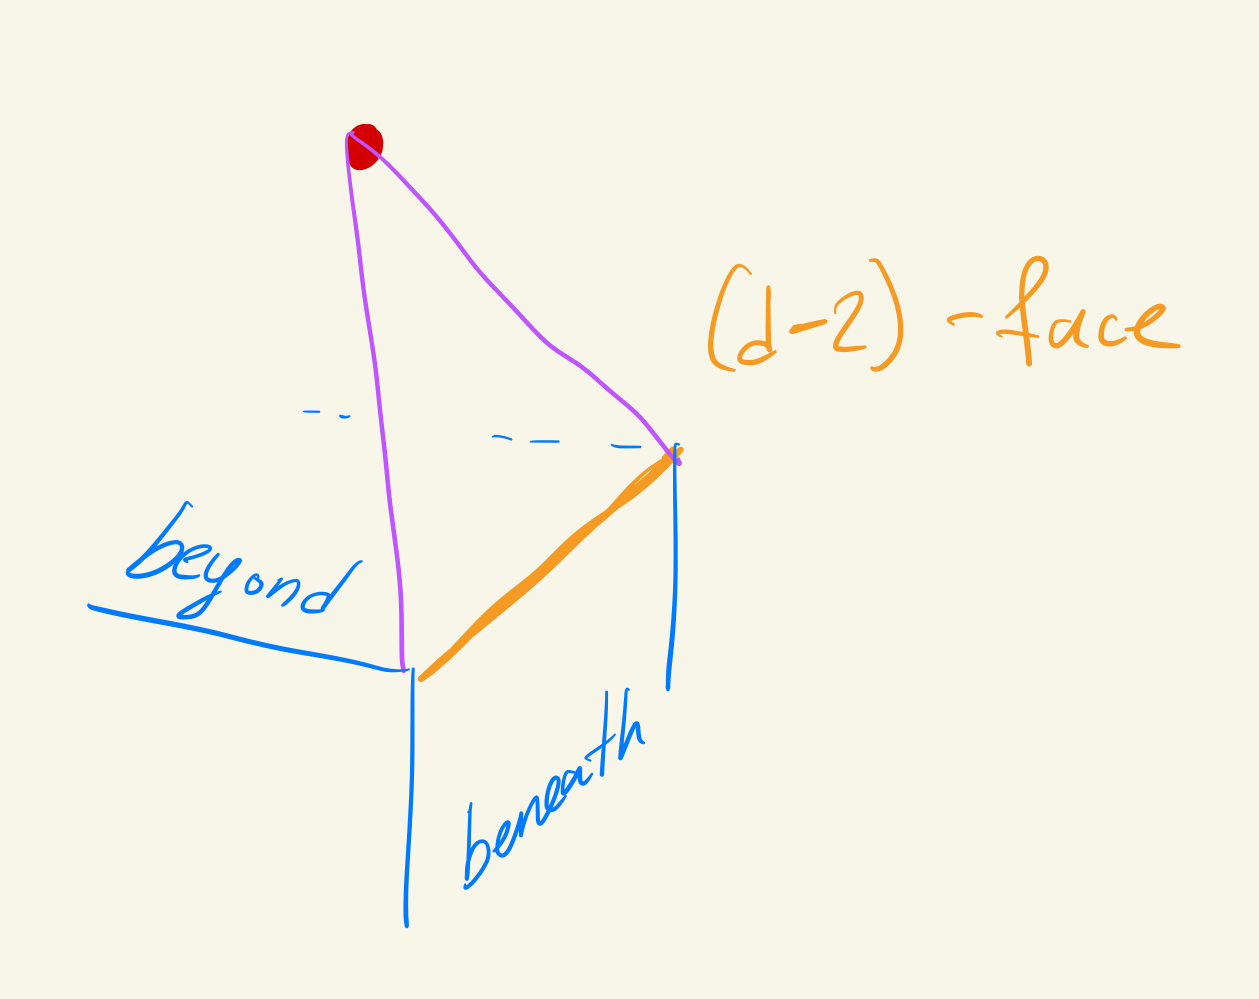
\includegraphics[width=0.3\textwidth]{fig6}
 	\caption*{The faces of \(P\) that contain \(V\)}
 \end{figure}
\begin{quotation}
	Therefore the combinatorial structure of \(P\) is completely determined by the combinatorial type of \(Q\) and the \((d-1)\)-complex \(\mathcal{C}\) consisting of those facets of \(Q\) beyond which \(V\) is, and their faces.
\end{quotation}
\begin{figure}[H]
	\centering
	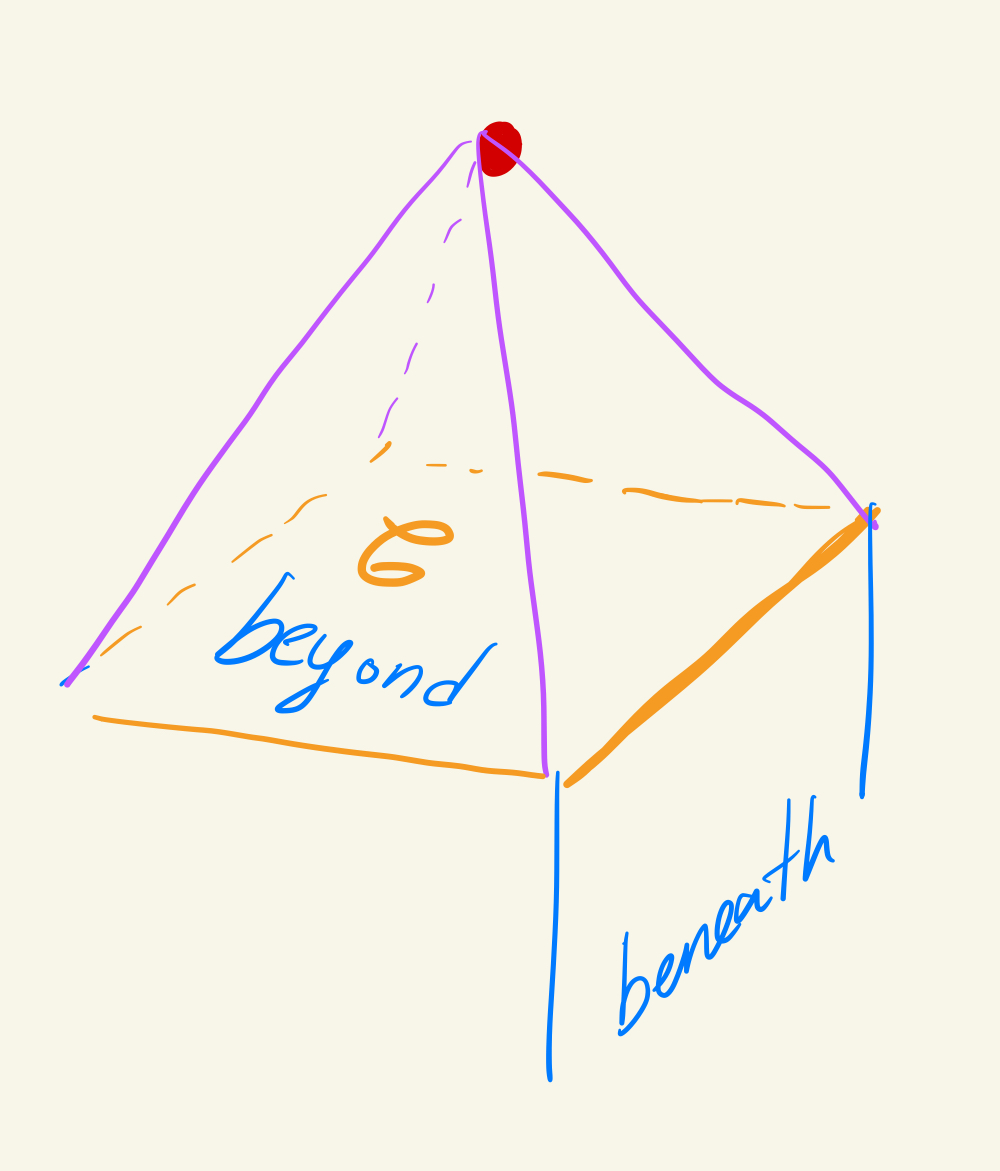
\includegraphics[width=0.3\textwidth]{fig7}
	\caption*{The complex \(\mathcal{C}\). It consists of the facets of \(Q\) beyond which \(V\) is.}
\end{figure}
The point here is that the classification of the \(P^8\)'s ends up being determined by the choice of \(P^7\) and the complex \(\mathcal{C}\) on its boundary. But there's a caveat in the construction:
\begin{quotation}
	One observation has to be borne in mind, however, in constructing the \(P^8\)'s from the \(P^7\)'s. […] with a given \(P^7\) and a complex \(\mathcal{C}\) on its boundary, there is, in principle, no guarantee for the existence of a point 8 that is beyond precisely those facets of \(P^7\) which are in \(\mathcal{C}\). For a given combinatorial type of \(P^7\), and a fixed \(\mathcal{C}\) on its boundary, such a point may exists, or may fail to exists […]. Hence, strictly speaking, what we have constructed so far are not 4-polyopes with 8 vertices, but certain combinatorial schemes, or 3-complexes, which may, or may not, be the boundary complexes of 4-polytopes.
\end{quotation}
Meaning that this construction, which seems intuitive and clear, may not be so natural in general. The resulting thing may not be geometrically what we expect, so it may not even be a polytope. And that's \(\mathcal{M}\)!

Indeed, in analyzing the different choices of complex \(\mathcal{C}\), Grünbraum and Shreedharan note first that the complexes \(\mathcal{A},\mathcal{B}_1,\mathcal{B}^2 \) and \(\mathcal{C}_2\) are of a certain type that ensures the existence of a vertex \(V\) that is beyond the facets of \(Q\) that are in any such \(\mathcal{C}\). Also the complexes \(\mathcal{C}_1\) and \(\mathcal{D}_1\) can be guaranteed to have an adequate vertex \(V\). The complexes \(\mathcal{C}_3\), \(\mathcal{D}_2\) and \(\mathcal{D}_3\) yield a combinatorially equivalent \(P^8\) to some of the former types, leaving only one complex to analyze, \(\mathcal{M}\).
\begin{quotation}
	``[…] as we shall now see, \(\mathcal{M}\) is indeed not combintorially equivalent to the boundary complex of any 4-poyltope. In other words, no representative of \(P_5^7\) has its facets in such a position that there exists a point \(V\) beyone precisely the facets of \(\mathcal{D}_3\)"
\end{quotation}



\iffalse
\begin{remark}\leavevmode
The greatest problem in the classification is to rule out the choices that give equivalent \(P\)'s.

In order to construct the classification,  Grünbraum and Sreedharan consider (1) the valence of the vertices, since the valence of \(V\) in \(P\) equals the number of vertices of \(\mathcal{C}\), (2) the fact that for a given \(P^7\), if there is a combinatorial morphism mappinc \(\mathcal{C}\) to \(\mathcal{C}'\), then the resulting \(P^8\)'s will be of the same combinatorial type (use Gale diagrams), and \((3)\) analyze the vertex figure at \(V\), which is a 3-polytope with at most 7 facets.

Considering these 3 remarks, Gru\&Sr conclude that only 9 complexes \(\mathcal{C}\) need to be considered for the classification, and they are listed in Table 2.
\end{remark}
\fi

\subsection{March 14: what's the valency of the vertices of \(\mathcal{M}\)?}

So, back to \cite{jan1}, I know that \(T^1_{A_{\mathcal{M}},0}\) is the \(\mathbb{C}\)-vector space on the edges of \(\mathcal{M}\) if \(\mathcal{M}\) is a combinatorial manifold without boundary and all vertices have valency greater than or equal to 5.

\begin{remark}\leavevmode
I'm not even sure that making sure whether the vertices of \(\mathcal{M}\) have or don't have valency \(\geq 5\) would help me at all: because what's the next step anyway?
\end{remark}

But here's the how this should be done: \(\mathcal{M}\) is constructed from \(P^7_5\) by choosing \(\mathcal{C}=\mathcal{D}_3\). So we could first have a look at the valency of the vertices in \(P^7_5\) and then at the valency of the vertices of the thing we obtain after doing the operation.

\subsection{March 19: wrap it up for a meeting with Galkin}

I find two main points of my work in this journal:
\begin{enumerate}
\item Keeping up the work on Grünbraum. Though progress has been slow, this topic remains fresh. I've been reading \cite{grun} lately, intending to understand the combinatorial structure of \(\mathcal{M}\). I think I could still get further on this task.

	But of course the question remains: even if I knew these combinatorics, what would I do next? The answer is what I could work on along with Galkin: understand what J. A. Christophersen has done.
	\begin{itemize}
	\item Deformation theory, SR schemes.
	\item Seems like there should be some toric geometry in all this. In the end, there's so much combinatorics… and indeed J. A. C. has used toric geometry to find the CY associated to the nicer triangulations…
	\end{itemize}
\item Understanding Fano varieties is also interesting. This is nicely linked with complex geometry à la Misha, since I can understand basic Fano variety theory in a complex-manifold context, using references I like like \cite{lec}, and of course pushing forward my knowledge on AG.

\item I didn't work on Pfaffian varieties lately.
\end{enumerate}

And here's what we could do: focus on understanding complex geometry, aiming, for example on deformation spaces, Kodaira-Spencer map, SR schemes. This has the double objective of preparating me for qualification exam (on the complex and algebraic geometry topics), while it remains a research topic.

If I was in a meeting with Galkin right now, I could explain the construction of the 8-vertex complexes from \cite{gru}.

\begin{thing8}{Preparation for Friday March 28}\leavevmode
\begin{enumerate}
\item (Objective.) Find a deformation of \(\mathbb{P}(\mathcal{K}_\mathcal{M})\) that is a CY3.
\item (Method.) Understand the deformation space of \(\mathbb{P}(\mathcal{K}_\mathcal{M})\).
\item (Main tool.) Kodaira-Spencer map from isomorphism classes of first order deformations and \(H^{1}(X,T_X)\). The description of tangent/cotangent sheaves is determined by combinatorics.
 \item (Current stage.) Understanding the combinatorial structure of \(\mathcal{M}\). Understanding elementary deformation theory (it's not elementary).
\end{enumerate}	
\end{thing8}

\subsection{March 31: how to find a smoothing within deformation space}

\begin{thing8}{Question}\leavevmode
How find a smoothing of a scheme, even knowing \(H^{1}(X,T_X)\)?
\end{thing8}

\begin{question}\leavevmode
What's the dimension of the simplicial complex \(\mathcal{M}\)? 3. What's interesting about it is that it is not the boundary of a 4-polytope--boundaries of 4-poyltopes have three dimensions. So that's why the smoothing would be a threefold.
\end{question}

\begin{question}\leavevmode
Why would \cite{jan1} get a CY3 from a triangulated torus i.e. a surface? This \textit{is} a mystery because after reviewing notes in this journal (search for ``construction of torus tiling") it indeed looks like the 
\end{question}

\begin{thing8}{Interesting remark}[\cite{jan1}, p.3]\leavevmode
Structure sheaf cohomology \(H^{p}(\mathbb{P}(\mathcal{K},\mathcal{O}_{\mathbb{P}(\mathcal{K})})\) is isomorphic to (most likely simplicial cohomology) \(H^{p}(\mathcal{K},\mathbb{C})\).
\end{thing8}

\begin{thing5}{Uninteresting remark}\leavevmode
	Notation in my talk the other day was actually wrong: \(\mathcal{K}\) usually means an arbitrary simplicial complex, while \(A_{\mathcal{K}}\) is the SR ring. So I should have put \(A_{\mathcal{M}}\) instead of \(\mathcal{K}_\mathcal{M}\).
\end{thing5}

\begin{thing8}{Interesting remark}[\cite{jan1}, p.3]\leavevmode
``If \(\mathcal{K}\) is an \textit{orientable}  combinatorial manifold then the canonical sheaf is trivial. Thus a smoothing of such a \(\mathbb{P}(\mathcal{K})\) would yield smooth schemes with trivial canonical bundle and the structure sheaf cohomology equaling \(H^{p}(\mathcal{K},\mathbb{C})\)."
\end{thing8}

So that one says… you are a CY! Well, almost, once again, what is a CY? A complex variety with trivial canonical bundle and… well for a K3 we would ask vanishing first structure sheaf cohomology. But for CY… actually just that---trivial canonical bundle.

\begin{thing4}{Uninteresting remark}\leavevmode
\cite{huc} has a chapter on deformations, but it looks like it's mostly about deformations of complex structures. No doubt it would be helpful to understand it, but at a first glance it might not be exactly what I'm looking for.
\end{thing4}

\begin{thing6}{Digression}[Calabi-Yau theorem interpretation inspired in \cite{huc} p. 226]\leavevmode
	Pick a compact Kähler manifold that admits a volume form. Also fix some \(\gamma \in H^{2}(X,\mathbb{C})\).  Then there is a Kähler metric with kahler form \(\omega\) such that \(\omega^n=\operatorname{Vol}\) and the curvature \([\omega]\) is \([\gamma]\).
\end{thing6}

\subsection{April 6: what's a triangle?}

\begin{thing8}{Epiphany}\leavevmode
the SR scheme of a simplicial complex is the simplicial complex in AG world. (I thought it was some mysterious scheme associated to the simplicial complex somehow.) 
\end{thing8}

\begin{thing6}{Exceptional case}\leavevmode
The simplex \(\Delta\) is different from all the rest because it has as many vertices as possible. That is, we are taking simplicial complexes to be subsets of the power set of as many vertices we like. And simplex simply has all the possible simplicices there are--it is the whole power set itself. So the SR ideal is empty, and the SR scheme is all projective space. So you have to take away the top face and consider only the codimension-1 faces if you want to see anything. So triangle SR ideal is \(\left<x yz\right>\).
\end{thing6}

\begin{exercise}[Deforming a triangle]\leavevmode
What's a triangle? A triangle is what you get after projecting to \(\mathbb{C}P^{2}\) the zero-set of the function \(f:\mathbb{C}^3 \to \mathbb{C}\) given by \(f(x,y,z)=xyz\). The differential fo this function is \(df=(yz,xz,xy)\) and will be zero at \((1,0,0),(0,1,0)\) and \((0,0,1)\); these are the vertices of the triangle. So a triangle is not a smooth manifold. But it can be smoothed if you consider \(f+tg\) for \(g=x^3+y^3+z^3\). You need the cubes because projective geometry (because if the polynomial is not homogeneous then the zero-set is not invariant under scaling and is not defined in the quotient \(\pi:\mathbb{C}^{3}\setminus\{0\}\to \mathbb{C}P^{2}\)). Have a look!

\begin{figure}[H]
	\centering
	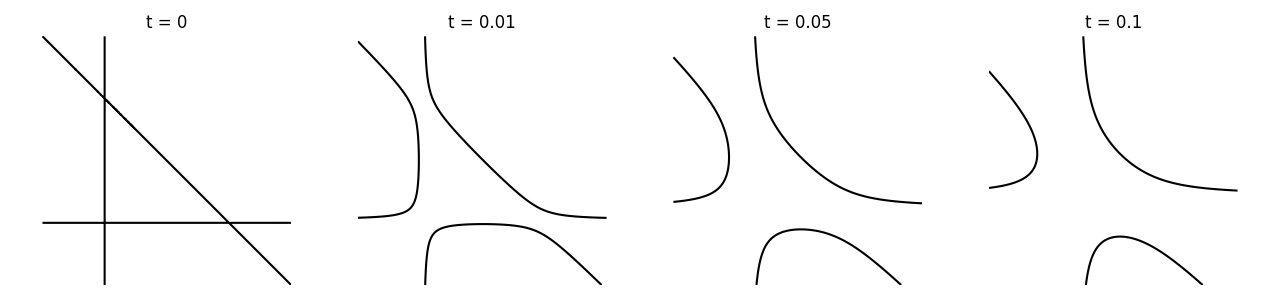
\includegraphics[width=0.9\textwidth]{fig8.png}
	\caption*{\(f+tg\)}
\end{figure}
\textbf{Note.} If you want to use this code again remember to remove the backslash before the underbars \_ on the .tex file.

\noindent\fbox{%
\begin{minipage}{\textwidth}
\texttt{%
import numpy as np\\
import matplotlib.pyplot as plt\\
\\
def f(x, y, t):\\
\ \ \ \ z = 1 - x - y\\
\ \ \ \ return x * y * z + t * (x**3 + y**3 + z**3)\\
\\
res = 400\\
x = np.linspace(-0.5, 1.5, res)\\
y = np.linspace(-0.5, 1.5, res)\\
X, Y = np.meshgrid(x, y)\\
\\
ts = [0, 0.1, 0.3, 1.0]\\
fig, axs = plt.subplots(1, len(ts), figsize=(16, 4))\\
\\
for i, t in enumerate(ts):\\
\ \ \ \ Z = f(X, Y, t)\\
\ \ \ \ axs[i].contour(X, Y, Z, levels=[0], colors='black')\\
\ \ \ \ axs[i].set\_title(f"t = \{t\}")\\
\ \ \ \ axs[i].axis('equal')\\
\ \ \ \ axs[i].axis('off')\\
\\
plt.tight\_layout()\\
plt.show()
}
\end{minipage}}
\begin{figure}[H]
	\centering
	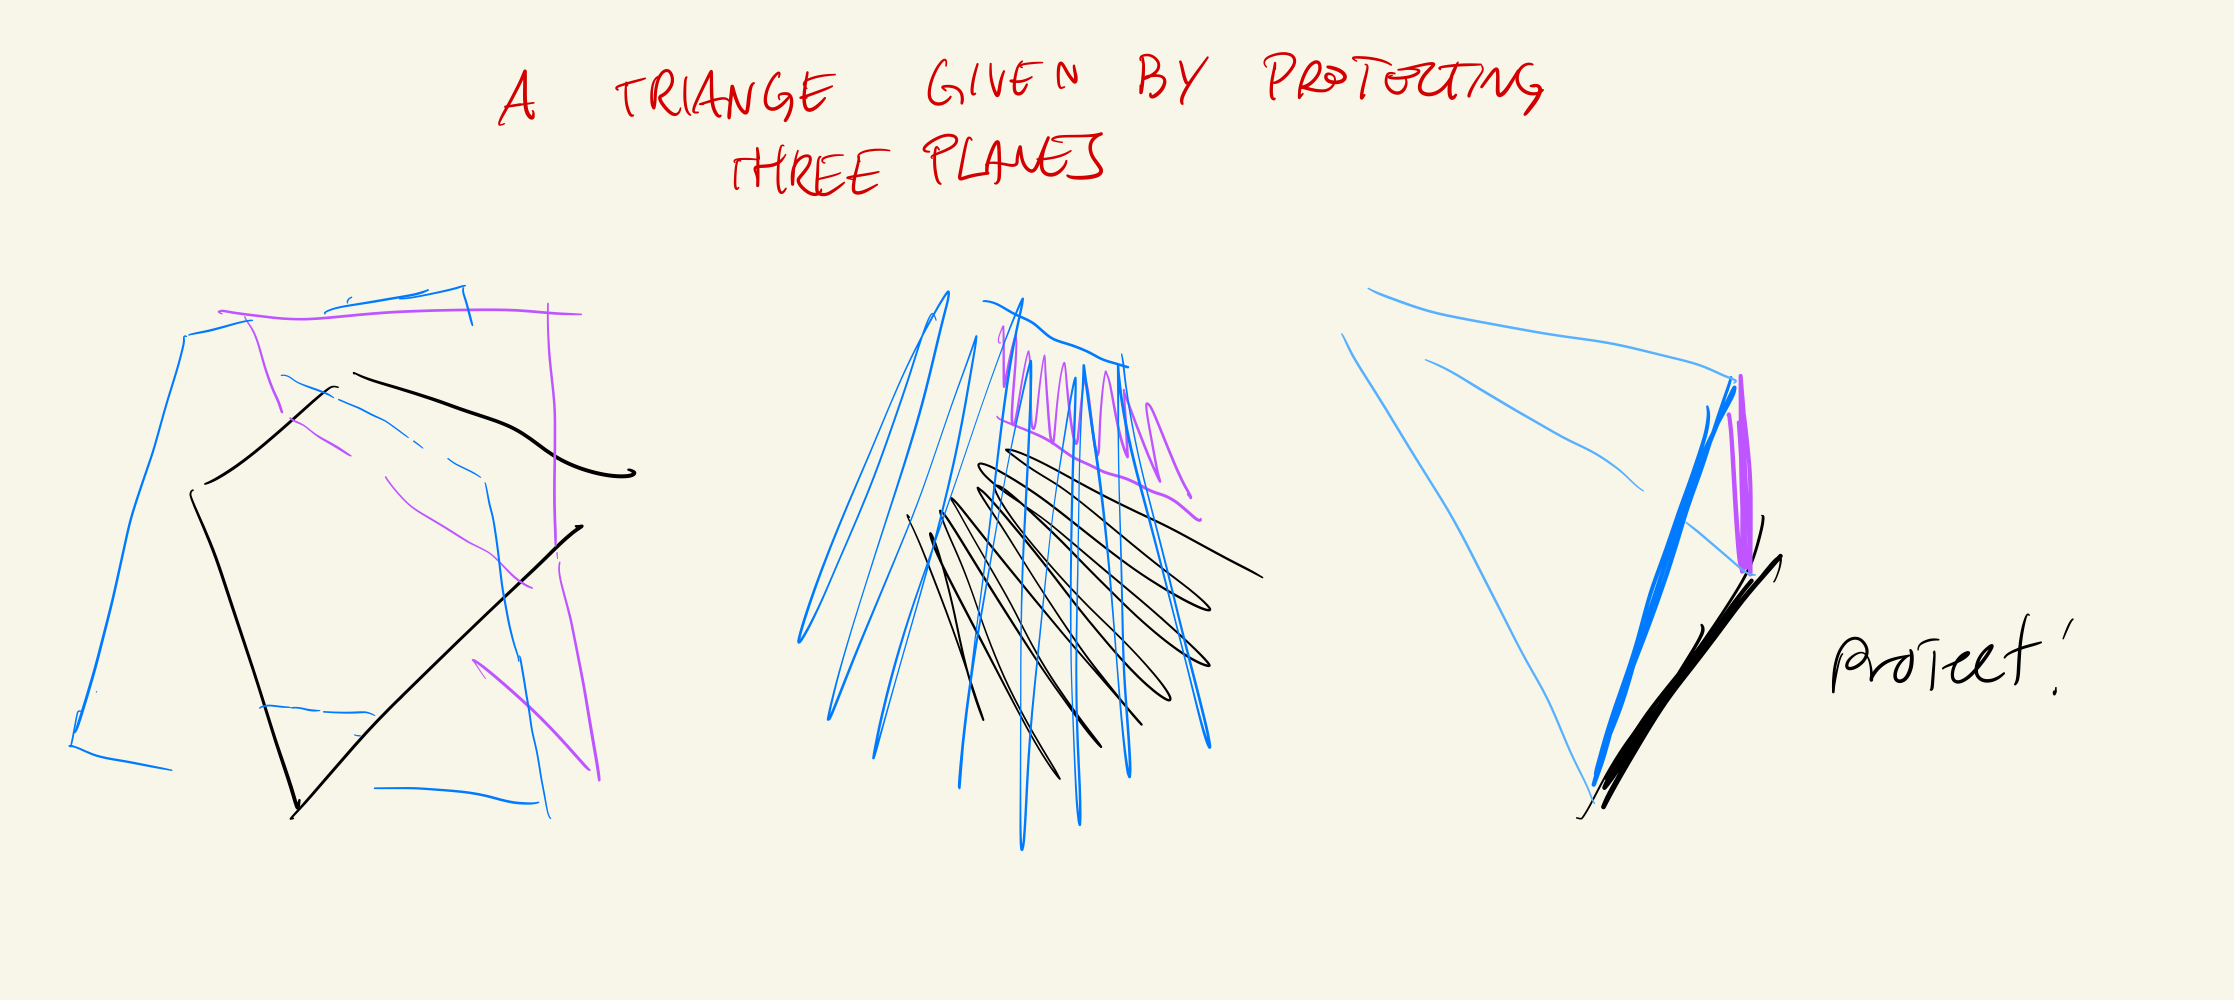
\includegraphics[width=0.9\textwidth]{fig9}
\end{figure}

\end{exercise}

\subsection{April 7: what are squares and pentagons}

\begin{thing8}{Example}[Square]\leavevmode
	A square is the projectivized zero-locus of the map \(f:\mathbb{C}^4 \to \mathbb{C}^2\) given by \(f(x,y,z,w)=(xz,yw)\). To understand what this zero-locus is just think that wither \(x=0\) or \(z=0\) and  \(y=0\) or  \(w=0\). This gives four options. When a variable is zero you are in a hyperplane orthogonal to the corresponding axis. So when two variables are zero (each of the 4 options) you are in the intersection of the corresponding two hyperplanes. Two hyperplanes intersect in a… 2-dimensional linear space. But when you go projective you get a line. So that's 4 lines, a square!

	Now the differential of  \(f\) is
	\[df=\begin{pmatrix} z & 0 & x & 0 \\ 0 & w & 0 y \end{pmatrix} \]
	which is singular when any three of the variables vanish, so that's the intersection of three hyperplanes, now that's a 1-dimensional thing in \(\mathbb{C}^4\), which is a point in the projective version. So there's 4 singular points, the corners of the square!

	Having said all that, I want a submersion \(g:\mathbb{C}^4\to \mathbb{C}^2\) to produce the smoothing \(f+tg\) so I want something like
	\[dg=\begin{pmatrix} x&y&z&w\\y&z&w&x \end{pmatrix} \]
	So I define
	\[g(x,y,z,w):=(x^2+y^2+z^2+w^2,xy+yz+zw+wx)\]
And I think it should work. Now there should be a way to draw this in \(\mathbb{R}^3\), because notice now that we are in \(\mathbb{C}P^3\), so there could be a visually nice representation of the smooth square. But ChatGPT couldn't do it so maybe later.	
\end{thing8}

Now what's a pentagon. That should be the first nontrivial example. But first here's some questions:

\begin{thing6}{Questions}\leavevmode
\begin{itemize}
\item The smoothing of a triangle is an elliptic curve (why?), but what is the smoothing of the square?
\end{itemize}
\end{thing6}

\begin{exercise}[Pentagon]\leavevmode
	So I define a map \(f:\mathbb{C}^5 \to \mathbb{C}^{\text{something} }\) where  \textbf{something} is the number of generators of the SR ideal, so the monomials corresponding to the simplices that are not in the pentagon. These are:
	\begin{itemize}
	\item Edges: 13,14,24,25,35
	\item Triangles: 123,124,125,234,235,345
	\end{itemize}
	So I have that \textbf{something} = 11. So the differential of \(f\) is a matrix with 5 columns and 11 rows. Writing it out, it \textit{looks} like there are five choices of vanishing variables \(x_i=0\) making the matrix singular. So it \textit{looks} like it is a pentagon. Just for the record let's put it here:
	\[df=\begin{pmatrix} x_3&0&x_1&0&0\\x_4&0&0&x_1&0\\0&x_4&0&x_2&0\\0&x_5&0&0&x_2\\0&0&x_5&0&x_3\\x_2x_3&x_1x_3&x_1x_2&0&0\\x_2x_4&x_1x_4&0&x_1x_2&0\\x_2x_5&x_1x_2&0&0&x_1x_2\\0&x_3x_4&x_2x_4&x_2x_3&0\\0&x_4x_5&0&x_2x_5&x_2x_1\\0&0&x_4x_5&x_3x_5&x_3x_4 \end{pmatrix} \]
And the point is that a smoothing is produce exactly like in the other rows by adding smartly functions at every coordinate among the 11 coordinate functions that \(f\) has making that matrix be nonsingular away from zero. So for example in the first row do what you need to do to get
\[\begin{pmatrix} x_3&x_2&x_1&x_4&x_5 \end{pmatrix} \text{ so you want }g_1=(0,x_2^2,0,x_4^2,x_5^2)\]
And so on. It's clear that such a \(g\) can be nicely constructed and we have a smoothing of the pentagon. Now what it is, I'm not sure.

\end{exercise}

\subsection{April 8: PUC Tuesday}

Things I wanted to discuss:
\begin{itemize}
\item Help with K3
\item Exercises on triangles and so on.	
\item Questions on Minimal surfaces: Explain the equation
	\[\operatorname{ Schild}(\varphi,\omega)=\int_{\Sigma}g du=\int \sqrt{g} \operatorname{Vol}_G\]
	and maybe also
	\[\operatorname{Symp}(\Sigma,\omega)=\int \omega\cdot \sum\left(\{x^i,x^j\}^2\omega\right) \]
And Dirichlet?
\item Working on twistors with Misha and others?
\item Didn't find Neron-Tate-Koadira.
\item  Reminder to send letter to Bridgeland stability
\end{itemize}

And the result was that we mostly discussed the triangles and squares and pentagon. The punchline is: \textbf{dani must learn what is complete intersection}. Becuase Pentagon is not complete intersection and that's why the computations I did don't work. So must understand this, must understand Bertini theorem. Second punchline is: you can and must use a computer to do computations and also you must learn to do computations without a computer.

There are some photos with evidence on all this.

\subsection{April 15: PUC from home Tuesday}

First a comment from Sergey on April 6 epiphany:

\begin{quotation}
	``One way to define the Stanley–Reisner (SR) scheme is as follows:

In \( V = \mathbb{R}^n \), consider a simplex \( \Delta \), given by the condition that the sum of coordinates is equal to 1.  
One interpretation is that \( \Delta \) is the simplex of probabilistic distributions on the set of \( n \) points,  
embedded in the cone of all measures on \( n \) points, which is a cone inside the vector space of all signed measures on this set (i.e., \( \mathbb{R}^n \)):

\[
\Delta \longrightarrow (\mathbb{R}_+)^n \longrightarrow \mathbb{R}^n
\]

Note that the image of \( \Delta \) does not contain the origin, so one can compose this embedding with the map \( \mathbb{R}^n \setminus \{0\} \to \mathbb{P}(\mathbb{R}^n) \).

Then, for any subcomplex \( K \subseteq \Delta \), consider the composition:

\[
K \longrightarrow \Delta \longrightarrow \mathbb{R}^n \longrightarrow \mathbb{P}(\mathbb{R}^n)
\]

The projective SR scheme \( \mathrm{SR}(K) \) is simply the Zariski closure in \( \mathbb{P}^{n-1} \) of the image of \( K \).  
Similarly, the affine SR scheme \( \mathrm{Cone}(\mathrm{SR}(K)) \) is the Zariski closure in \( \mathbb{A}^n \) of the image (in \( \mathbb{R}^n \)) of the cone over \( K \) with vertex at 0."
\end{quotation}
How to apply this idea?

And then there's the whole thing on resolutions. This is the correct way to deform schemes, and what should be discussed with Victor. Here's some key points I'd like to clarify:

\begin{itemize}
\item (Preliminary) What's the structure sheaf of a variety.
\item What's a resolution of the structure sheaf.
\item What's a resolution of the structure sheaf of a complete intersection. Koszul complex. Example: a ``triangle", \(V(xyz) \subset \mathbb{P}^\).
\item What's a resolution of the structure sheaf of a non complete intersection. Example: three points in \(\mathbb{P}^2\), \([1:0:0],[0:1:0],[0:0:1]\).
\item Extra: example of \(\operatorname{Gr}(2,5)\) in Plücker embedding and it's relation with Pentagon.
\end{itemize}

So probably this last point should lead to the correct smoothing of the pentagon. Of course, independently of all this I should understand what went wrong in the computations from last week (regarding the pentagon).

Actually look, I think the case of the pentagon was written by Galkin two Tuesdays ago:
\[\begin{tikzcd}
	0\arrow[r]& K\arrow[r]&\mathcal{O}(-2)^{\oplus 5}\arrow[r,"\begin{pmatrix} x_1x_2\\x_2x_4\\\vdots \\x_5x_2 \end{pmatrix} "]&\mathcal{O}_\mathbb{P}\arrow[r]&0
\end{tikzcd}\]
So yes, that map in the middle is a matrix composed of the polynomials that determine the variety (which is not a complete intersection).

\subsubsection{Corrections on pentagon}

\begin{question}\leavevmode
Why does my approach to smoothing the pentagon not work?
\end{question}

Let's go over what happened. I first did the triangle case:

\begin{quotation}
	``What's a triangle? A triangle is what you get after projecting to \(\mathbb{C}P^{2}\) the zero-set of the function \(f:\mathbb{C}^3 \to \mathbb{C}\) given by \(f(x,y,z)=xyz\). The differential of this function is \(df=(yz,xz,xy)\) and will be zero at \((1,0,0),(0,1,0)\) and \((0,0,1)\); these are the vertices of the triangle. So a triangle is not a smooth manifold. But it can be smoothed if you consider \(f+tg\) for \(g=x^3+y^3+z^3\), whose differential is not zero away from zero. You need the cubes because projective geometry (because if the polynomial is not homogeneous then the zero-set is not invariant under scaling and is not defined in the quotient \(\pi:\mathbb{C}^{3}\setminus\{0\}\to \mathbb{C}P^{2}\)). Have a look! *has a look*"
\end{quotation}

And then I went on to square (skip for now) and then to pentagon. First mistake was that I considered too many functions to define the pentagon. \(\mathsf{OK}\) let's think about this: to produce the SR ideal we have a look at the simplices that are not in the simplex which are, as I noticed,
\begin{itemize}
	\item Edges: 13,14,24,25,35
	\item Triangles: 123,124,125,234,235,345
\end{itemize}
But then what? That the ideal \((x_1x_2x_3)\) is contained in the ideal \((x_1x_3)\) so \(k[x_1,\ldots,x_5]/(x_1x_3,x_1x_2x_3)=k[x_1,\ldots,x_5]/(x_1x_3)\). So you didn't need to include the triangles. And then what happened is that you just didn't know how to check for situations in which the differential is singular. (Recall from dif top that a map is singular if \(\operatorname{corank}=\operatorname{min}(\dim \text{domain},\dim \text{codomain})  -\operatorname{rk} df\) is positive, so in this case if \(df\) has rank less than 5.) \(\mathsf{OK}\) so here's the matrix:
	\[df=\begin{pmatrix} x_3&0&x_1&0&0\\x_4&0&0&x_1&0\\0&x_4&0&x_2&0\\0&x_5&0&0&x_2\\0&0&x_5&0&x_3\end{pmatrix} \]

So what happened is basically that I forgot how to compute the rank of a matrix. Recall that rank is the number of linearly independent columns… and, if you recall, a \(5 \times 5\) matrix would have rank less than 5 \(\iff\) \(\det =0\). So you want the determinant. That's when computers come in handy. GPT says: \(\det=-2x_1x_2x_3x_4x_5\).

So the rank is less than 5 when any of the coordinates is zero. So in the union of the 5 coordinate hyperplanes of \(\mathbb{C}^5\). Projectivize, and you'll get a singular locus of \(5\) hyperplanes of \(\mathbb{C}P^{4}\). So where's the pentagon? I think you find the pentagon when you intersect the projectivization of the zero set of \(f:\mathbb{C}^5\to \mathbb{C}^5\) (i.e. the projective variety) with any 2-dimensional plane in \(\mathbb{C}P^{6}\).

Right, so after long discussions with GPT we have come to the conclusion that this scheme \(X\) is entirely singular. Because the determinant will be zero if any of the of the coordinates of a point are zero, but guess what: all points of \(X\) must have at least one coordinate that is zero. Of course because by definition, points of \(\mathbb{P}^4\) are in \(X\) when:
\[x_1=0\text{ or } x_3=0\quad\text{and}\quad   x_1=0\text{ or } x_4=0\qquad \text{ etc} \]
So in particular some coordinate must be zero. So all the points of \(X\) are singularities. What's going on?

Also, the so-called naive smoothing \(f+tg\) doesn't work for reasons probably related to the strangeness of \(X\), related to the fact that it is not a complete intersection (=codimension of the variety is not the number of generators of the ideal).

\subsubsection{Since pentagon is already too complicated…}

we consider a non-complete intersection that is the simplest case ever. It's the following combinatorial simplicial complex:
\[\begin{tikzcd}
	\bullet\arrow[r,no head]&\bullet\arrow[r,no head]&\bullet\arrow[r,no head]&\bullet
\end{tikzcd}\]
Quickly! What's the SR scheme associated to this simplicial complex? It lives in \(\mathbb{P}^3\), and I guess the SR ideal is just \((x_1x_3,x_1x_4,x_2x_4)\). Before looking at singularities let me think: what is this? It's a union of some lines in \(\mathbb{P}^3\), \(x_1=0 \cap x_2=0\), \(x_1=0 \cap x_4=0\) and \(x_3=0 \cap x_4=0\). Right, it matches the drawing above (phew!). Singularities are whenever the matrix
 \[\begin{pmatrix} x_3&0&x_1&0\\x_1&0&0&x_1\\0&x_4&0&x_2 \end{pmatrix} \]
has rank less than… 3. Sooo, probably there's two singularities right?

GPT \textit{kind of concludes} that either \(x_1=0\) or \(x_1\neq 0\) and \(x_2=x_4=x_2\). But it's suspicious---he gave different answers when I asked the same question. I'm quite convinced it's right though. \(\mathsf{OK}\) let's just put the computations from GPT so we are all sure about this:

We consider the matrix
\[
A = \begin{pmatrix} 
x_3 & 0   & x_1 & 0 \\
x_1 & 0   & 0   & x_1 \\
0   & x_4 & 0   & x_2 
\end{pmatrix}
\]
which is of size $3 \times 4$, so its rank is at most 3. We want to determine when it has rank strictly less than 3. This occurs exactly when all $3 \times 3$ minors vanish.

We compute the $3 \times 3$ minors:
\begin{align*}
\det A_{123} &= 
\begin{vmatrix}
x_3 & 0   & x_1 \\
x_1 & 0   & 0   \\
0   & x_4 & 0
\end{vmatrix}
= x_1^2 x_4 \\
\det A_{124} &= 
\begin{vmatrix}
x_3 & 0   & 0 \\
x_1 & 0   & x_1 \\
0   & x_4 & x_2
\end{vmatrix}
= -x_1 x_3 x_4 \\
\det A_{134} &= 
\begin{vmatrix}
x_3 & x_1 & 0 \\
x_1 & 0   & x_1 \\
0   & 0   & x_2
\end{vmatrix}
= -x_1^2 x_2 \\
\det A_{234} &= 
\begin{vmatrix}
0   & x_1 & 0 \\
0   & 0   & x_1 \\
x_4 & 0   & x_2
\end{vmatrix}
= -x_1^2 x_4
\end{align*}
Hence, all $3 \times 3$ minors vanish if and only if
\[x_1 = 0 \quad \text{or} \quad (x_1 \neq 0 \text{ and } x_2 = x_4 = 0).\]
\(\mathsf{OK}\), and then: what is this? Either the hyperplane \(x_1=0\) or the line \(x_2=x_4=0\). Superstrange. Again. And then we say whoa, again, all the points of this scheme are singular! Because to be in the scheme either \(x_1=0\) or \(x_4=0\). So it's kind of the same as in the pentagon case.

But there's no substantial difference that would tell me how to smooth either the pentagon or this other scheme. Or let alone smooth, maybe start by understanding the algebraic geometry of these things.

\subsection{Summoning Victor}

Here's a short text to be read by Victor before a potential meeting.

Objective of meeting: understand deformation of schemes using resolutions of structure sheaf.

\begin{itemize}
	\item \textbf{(Preliminary) What's the structure sheaf of a variety.} Maybe skip, or just define elementary concepts to be used in practice.
	\item \textbf{What's a resolution of the structure sheaf.} I don't know a lot about this but let me say what I do know. I recall from Voisin, last year when I did some notes on de Rham/Dolbeault theorem that a resolution of a sheaf is an exact sequence starting with the sheaf. So for example a resolution of the constant sheaf \(\underline{\mathbb{R}}\) is the complex of sheaves of differential forms of degrees up to the dimension of the manifold. Then de Rham theorem is essentially proved when we realize that the singular chain complex is \textit{also} a resolution of the constant sheaf \(\underline{\mathbb{R}}\). Poincaré lemma is what assured us that the de Rham complex is a complex, i.e. \(\ker \subset \operatorname{img}\) because locally closed forms are exact. We also had Dolbeault complex for \(\overline{\partial}\).
	\item \textbf{What's a resolution of the structure sheaf of a complete intersection.} Koszul complex. I don't know this. This and the next item are what we should really focus on. Ideally we could apply this item, i.e. complete intersection case, to the following example of a Stanley-Raisner scheme (at the end of this document I put some definitions about SR things): 
\begin{example}\leavevmode
What's a triangle? A triangle is what you get after projecting to \(\mathbb{C}P^{2}\) the zero-set of the function \(f:\mathbb{C}^3 \to \mathbb{C}\) given by \(f(x,y,z)=xyz\). The differential fo this function is \(df=(yz,xz,xy)\) and will be zero at \((1,0,0),(0,1,0)\) and \((0,0,1)\); these are the vertices of the triangle. So a triangle is not a smooth manifold. But it can be smoothed if you consider \(f+tg\) for \(g=x^3+y^3+z^3\). You need the cubes because projective geometry (because if the polynomial is not homogeneous then the zero-set is not invariant under scaling and is not defined in the quotient \(\pi:\mathbb{C}^{3}\setminus\{0\}\to \mathbb{C}P^{2}\)). Have a look!

\begin{figure}[H]
	\centering
	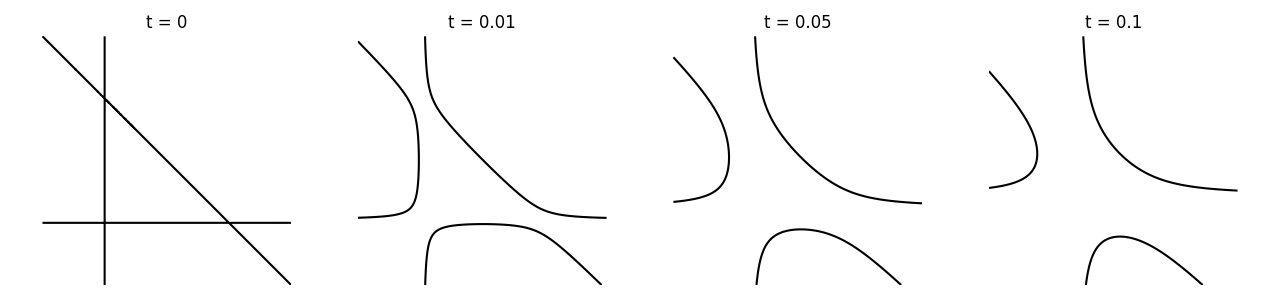
\includegraphics[width=0.9\textwidth]{fig8.png}
	\caption*{\(f+tg\)}
\end{figure}
\end{example}	

\item \textbf{What's a resolution of the structure sheaf of a non complete intersection.} This is where it becomes tricky: I've been trying to understand the example of the SR scheme associated to a pentagon but I get some weird results like that the whole scheme is its singular locus (I'm not sure whether this is correct and even less how to construct a smoothing; the same trick of defining \(f+tg\) shouldn't work). Easier than for the pentagon, we could work on the resolution of the (Stanley-Raisner) scheme composed of three points in \(\mathbb{P}^2\), \([1:0:0],[0:1:0],[0:0:1]\).
\item \textbf{Finally:} we could get closer to the pentagon if we work on the example of \(\operatorname{Gr}(2,5)\) in Plücker embedding. (Sergey has mentioned it's related to the pentagon.) (Also Sergey once wrote som following on a board:
	\[\begin{tikzcd}
	0\arrow[r]& K\arrow[r]&\mathcal{O}(-2)^{\oplus 5}\arrow[r,"\begin{pmatrix} x_1x_3\\x_2x_4\\\vdots \\x_5x_2 \end{pmatrix} "]&\mathcal{O}_\mathbb{P}\arrow[r]&0
\end{tikzcd}\]
\end{itemize}
(The SR scheme associated to the pentagon is given by the ideal \((x_1x_3,x_1x_4,x_2x_4,x_2x_5,x_3x_5)\).) Anyway that is just to say we are looking for these kind of complexes where the maps are given by matrices. Looks like this is the right way to smooth SR schemes.

\vspace{1em}
Finally I include some basic theory of SR schemes just for context of what I'm doing. Recall that my ultimate objective is to smooth a SR scheme coming from specific complex (which is not mentioned here at all).

		Let $[n]$ be the set of all positive integers from 0 to $n$, and let $\Delta_n$ denote the power set of $[n]$. A subset $K\subseteq \Delta_n$ we call \textit{\textbf{simplicial complex}} if for every $f\in K$ all the subsets of $f$ are also in $K$. Let $P=k[x_0,\ldots,x_n]$ be a polynomial ring in $n+1$ variables over an algebraically closed field $k$. If $a=\{i_1,\ldots,i_k\} \in\Delta_n$ then we write $x_a\in P$ for the square free monomial $x_{i_1}\cdot \ldots\cdot x_{i_k}$. A simplicial complex $\mathcal{K}\subset \Delta_n$ gives rise to the ideal
		\[I_{\mathcal{K}}:=\left<x_a: a\in\Delta_n\setminus \mathcal{K}\right> \subseteq P\]
		that is, the \textit{\textbf{Stanley-Reisner ideal}} is generated by the monomials that that are \textit{not} in the polytope. The \textit{\textbf{Stanley-Reisner ring}} is $A_{\mathcal{K}}:=P/I_{\mathcal{K}}$. We associate an affine scheme $\mathbb{A}(\mathcal{K}) =\operatorname{Spec}(A_{\mathcal{K}})$ and projective scheme $\mathbb{P}(\mathcal{K})=\operatorname{Proj}(A_{\mathcal{K}})$, the latter called the \textit{\textbf{Stanley-Raisner scheme}}.


\clearpage
\section{Pfaffian varieties}

{\color{2}Here's some context on how the Pfaffian journey started:}

\begin{thing4}{Dani}[October 14]\leavevmode
	We had also briefly discussed deformations of Pfaffian threefolds and their relation to tropical varieties {\color{3}[This happened in August]}. I have read a (very) little about Pfaffian threefolds, but still not about their relation to tropical varieties or to the search of a CY3 from Grünbaum sphere.
\end{thing4}

\begin{thing14}{Sergey}[October 15]\leavevmode
	Pfaffian threefolds per se are not more related to tropical varieties than any other threefolds. Tropical varieties are related to tropical deformations/degenerations of everything, here Pfaffian is just an interesting example to apply the machinery of tropical and SR things. Alex and Victor and Altan know a bit about Pfaffian varieties, in particular about Grassmannian/Pfaffian correspondence.
\end{thing14}

\subsection{Reading \cite{pfaffian}}

{\color{2}So in that message this is what I meant when I said "I have read a (very) little about Pfaffian threefolds"}

\begin{thing4}{Pfaffian Threefolds in Projective space}\leavevmode
	Suppose that $R$ is a regular local ring and $I\subset R$ is an ideal of height 1 or 2. J. P. Serre proved that $R/I$ is Gorenstein if and only if it is complete intersection. This is no longer true for height 3 ideals, but such Gorenstein ideals are characterized as pfaffian ideals of certain skew-symmetric matrices.
\end{thing4}

{\color{persimmon}Yes! I remember this had to do with skew-symmetric matrices. That day when I talked to Sergey I was just starting to study symplectic vector spaces (first steps in symplectic geometry course). I don't remember exactly what he said, but I guess that the determinant of a skew-symmetric matrix is $\pm 1$.}

\begin{thing4}{Pfaffian Threefolds in Projective space}[Cont.]\leavevmode
	This observation suggests tha pfaffian verieties form a reasonable class of varieties to study when we investigate non-complete intersection Gorenstein varieties. In this subsection we review the basics of pfaffians in order to make this paper self-contained.
\end{thing4}

Thgoughout this paper we work over the complex numbers $\mathbb{C}$. Let $\operatorname{SkewSym}(n,\mathbb{C})$ be the set of $n\times n$ skew symmetric matrices. For $N=(n_{i,j}\in\operatorname{SkewSym}(n,\mathbb{C})$, the \textit{\textbf{pfaffian}} is
 \[\operatorname{Pf}(N)=\frac{1}{r!r^r}\sum_{\sigma\in\mathfrak{S}_{2r}}\operatorname{sign}(\sigma) \prod_{i=1}^rn_{\sigma(i)\sigma(r+i)}  \]
 if $n=2r$ is even and 
  \[\operatorname{Pf}(N)=0\]
  if $n$ is odd. {\color{persimmon}So, a polynomial, right?}

*Some other considerations related to adjoint matrix and determinant of $N$*

\begin{thing2}{\href{https://en.wikipedia.org/wiki/Pfaffian}{Wiki}}\leavevmode
	In mathematics, the determinant of an  $m\times m$ skew-symmetric matrix can always be written as the square of a polynomial in the matrix entries
	\[\operatorname{Pf}(A)^2=\det(A),\]
a polynomial with integer coefficients that only depends on $m$. When $m$ is odd, the polynomial is zero, and when $m$ is even, it is a nonzero polynomial of degree $\frac{m}{2}$, and is unique up to multiplication by $\pm 1$. {\color{persimmon}There has to be some convention taken to establish the exact definition of pfaffian.} The value of this polynomial, when applied to the entries of a skew-symmetric matrix is called the \textit{\textbf{Pfaffian}} of that matrix. The term Pfaffian was introduced by Cayley (1852), who indirectly named them after Johan Friedrich Pfaff.
\begin{figure}[H]
	\centering\hfill
	
\includegraphics[width=0.05\textwidth]{fig2.png}
	\caption*{\hfill {\tiny Pfaff}}
\end{figure}
\begin{quotation}
	They asked Laplace who, in his opinion, was the greatest mathematician of Germany. "It's Pfaff," he answered.

	He studied mathematical series and integral calculus, and is noted for his work on partial differential equations of the first order Pfaffian systems, as they are now called, which became part of the theory of differential forms; and as Carl Friedrich Gauss's formal research supervisor. He knew Gauss well, when they both lived together in Helmstedt in 1798. August Möbius (from the Möbius strip) was later his student.
\end{quotation}
\end{thing2}

\begin{prop}\leavevmode
	For a $2n\times 2n$ skew-symmwtric matrix $A$,
	\begin{itemize}
	\item $\operatorname{Pf}(A^{\mathbf{T}})=(-1)^n\operatorname{Pf}(A)$ 
	\item $\operatorname{Pf}(\lambda A)=\lambda^n\operatorname{Pf}(A)$ 
	\item $\operatorname{Pf}(A)^2=\det A$ 
	\item $\operatorname{Pf}(BAB^{\mathbf{T}})=\det B\operatorname{Pf}(A)$ for arbitrary $2n\times 2n$ matrix $B$.
	\item $\operatorname{Pf}(A^{2m+1})=(-1)^{nm}\operatorname{Pf}(A)^{2m+1}$
	\end{itemize}
\end{prop}

\begin{thing1}{Other properties}\leavevmode
	\begin{itemize}
	\item Pfaffian is an invariant polynomial of a skew-symmetric matrix under proper orthogonal change of basis (remember \cite{tud}). As such, it is important in the thoery of characterstic classes. In particualr, it can be used to define the Euler class of a Riemannian manifold that used in the generalizaed Gauss-Bonnet theorem.
	\item To calculate number of domino tilings.
	\end{itemize}
\end{thing1}

{\color{persimmon}Back to \cite{pfaffian}}

Let us first recall the construction of pfaffian varieties in $\mathbb{P}^n$, $n>3$.

{\color{persimmon}This part is certainly harder. Looks like the objective is to dine a map $P$ such that}

\begin{defn}
	A projective variety $X\subset \mathbb{P}^n$ is called the \textit{\textbf{pfaffian variety}} associated to  $(t,\mathcal{E},N)$ if the structure sheaf $\mathcal{O}_X$ is given by $\operatorname{coker} P$. The sheaf $\operatorname{img} P\subset \mathcal{O}C_{\mathbb{P}^n}$ is called the \textit{\textbf{pfaffian ideal sheaf}} of $X$ and denoted $\mathcal{I}_X$.
\end{defn}

{\color{persimmon}$\operatorname{OK}$ so what is $(t,\mathcal{E},N)$}

Given an integer $t\in\mathbb{Z}$ and a locally free sheaf $\mathcal{E}$ {\color{persimmon}(=vector bundle?)} of odd rank $2r+1$ on  $\mathbb{P}^n$, a global section $N\in H^{0}(\mathbb{P}^n,\Lambda^{2}(\mathcal{E}(t)))$ {\color{persimmon}(=2-form on $\mathcal{E}$?)} defines an alternating morphism $\mathcal{E}^\vee \overset{N}{\longrightarrow}\mathcal{E}$ {\color{persimmon}(this $\mathcal{E}^\vee (-t)$ is the twisted bundle which I'm currently not so sure what it is…)}. The pfaffian complex associated to $(t,\mathcal{E},N)$ is given by
\[\begin{tikzcd}
0\arrow[r]&\mathcal{O}_{\mathbb{P}^n}(-t-2s\arrow[r]&\mathcal{E}^\vee (-t-s)\arrow[r]&\mathcal{E}(-s)\arrow[r]&\mathcal{O}_{\mathbb{P}^n}
\end{tikzcd}\]
where $s=c_1(\mathcal{E})+rt$ and$P$ is defined as
\[P=\frac{1}{r!}\wedge^rN \in H^{0}(\mathbb{P}^n,\wedge^{2r}\mathcal{E}(rt))\]
The first and third morphisms are fiven by taking the wedge product with $P$ and $P^{t}$ respectively. Once we fix a basis of sections $e_1,\ldots, e_{2r+1}$ of $E$, $N$ may be expressed as a matrix and then $P$ is just given by
\[P=\sum_{i=1}^{2r+1}\operatorname{Pf}(N_i)\bigwedge_{j\neq 1}e_j.\]

{\color{persimmon}It goes on to some degeneracy locus, $X$ locally Gorenstein, $X$ pfaffian Calaby-Yau,}
\begin{quotation}
	in his paper [17], F. Tonoli constructed pfaffian Calabi-Yau threefolds for degree $d$ in the range $11\leq d \leq 17$.
\end{quotation}
{\color{persimmon}Other comements,…}
\begin{quotation}
	It is verified that $X_{14}$ and its mirror partner $\check{X}_{14}$ have rich mathematic structures in [14,4,12]
\end{quotation}

\subsection{Discussion in Telegram}

\begin{thing3}{Altan}\leavevmode
Isn't Pfaffian just the determinantal subvarieties in skew-symmetric matrices?  Just the set of $A$ in $\mathcal{M}_{n\times n}$ such that $A + A^{\mathbf{T}} = 0$ and $\operatorname{rk} A = r$.
\end{thing3}

\begin{thing1}{Dani}\leavevmode
	Sounds like a good description… but I couldn’t tell so far. I had read that a projective variety is called Pfaffian when its structure sheaf is given by the cokernel of a certain Pfaffian map. The Pfaffian of a skew-symmetric matrix is a root of its determinant
\end{thing1}

\begin{thing4}{Sergey}\leavevmode
	There are many things that can be called Pfaffian vareties.

	One thing is $\operatorname{rk} A = r$ usually is often not Zariski closed, need $\operatorname{rk} A \leq  r = 2k$.

Second thing is what are the entries of the matrix $A$.

Third thing - in which sense $A$ is a matrix (as Dani writes, it can be a morphism between vector bundles).
\end{thing4}

\begin{thing3}{Altan}\leavevmode
	1. Sure.  Same game as for determinantal varieties.

2. Idk, complex numbers?

3. For me it is just a matrix in the most naive sense; but nothing permits us from executing the construction over some base, as you are saying.  The question is why would we do it.
\end{thing3}

 \begin{defn}[Sergey]\leavevmode
 	Data for \textit{\textbf{Pfaffian subvariety}} is:
	\begin{itemize}
	\item A vector bundle $E$,
	\item a line bundle $ L$, and
	\item an $L$-valued endomorphism of $E$, which is skew symmetric. {\color{4}\textbf{Exercise}: define what this means.}
	\end{itemize}
	With this data you associate a subvariety of the locus of points on $ X$ where rank is at most $2k$.
 \end{defn}

 \begin{example}\leavevmode
 	If  $r=2k+3$, then this is a codimension 3 subvariety. And nobody knows any interesting construction of codimension 3 subvarieties (e.g. in $\mathbb{P}^6$) other than this one.
 \end{example}

 \begin{conjecture}[Hartshorne]
 	Codimension 3 in $\mathbb{P}^n$ are c.i. for $n\geq 10$.
\end{conjecture}

\begin{proof}[Solution]\leavevmode
	$\mathsf{OK}$ so I think we have a manifold $X$, and a vector bundle $E$ so to every point $x \in X$ put a vector space $E_x$ and a line bundle  $L$ that puts a line $L_x\cong k$ in every point. So an $L$-valued endomorphism of $E$ is a bundle map
	\[\begin{tikzcd}
	E\arrow[rr,"\varphi"]\arrow[dr,"p_1",swap]&&E\arrow[dl,"p_1"]\\
	&X
	\end{tikzcd}\]
	but what does it mean that it is $L$-valued? That  for every $(x,e)\in E$, $\varphi(x,e)\in L_x$ maybe? Or maybe in $L_{\varphi(x)}$, no because since $\varphi$ is a bundle map then it commutes with projections so it doesn't move the base---it is a linear isomorphism of fibers. So I think that $L_x\subset E_x$ and then $\varphi$ puts $E_x$ in  $L_x$ so it's kind of a contracting map because puts the vector space  $E_x$  on a line.

	So skew-symmetry doesn't mean anything unless we make the bundle map be a bilinear map. So I want something like
	\[\begin{tikzcd}
	E\times E\arrow[rr,"\varphi"]\arrow[dr,"p_1\times p_1",swap]&&L\arrow[dl,"p_L"]\\
	&X
	\end{tikzcd}\]
	which perhaps, and only perhaps, may be related to something like perfect pairin, giving some map $E\to  E^*$. So \href{https://en.wikipedia.org/wiki/Pairing#Definition}{wiki}:a  \textit{\textbf{pairing}} of  $R$-modules $M$,  $N$,  $L$ is an $R$-linear map $M\otimes_R N\to L$  and can also be considered as an $R$-linear map $M \to \operatorname{Hom}(N,L)$. A pairing is called \textit{\textbf{perfect}} if the latter map is an isomorphism. A pairing is called  \textit{\textbf{alternating}} if $N=M$ and  $(m,m)\mapsto 0\;\forall m$, which implies that $\varphi(m,n) =-\varphi(m,n)$. ($\varphi$ is the pairing. . .)

	So I think we consider the pairing map
	\[E\to \operatorname{Hom}(E,L)\]
	and look for its rank. And then the Pfaffian is the locus of degeneracy of this map, or bettery yet the locus where the map is of rank at most $r$. So {\color{8}perhaps $r$ is odd? In Sergey's comment (see  \cite{luk2}).}

		{\color{8}Write this correctly and send to group.}
\end{proof}

\vspace{1em}

 And here's some objectives (also a message from Sergey):

\begin{itemize}
\item What is a Pfaffian CY3 in Grassmannian/Pfaffian correspondence
\item What is Pfaffian representation of a cubic hypersurface, in which dimensions it always exist, in which not, what is the variety of Pfaffian representations
\item Papers by Kapustka and by Kanazawa on classification of other Pfaffian CY3.
\item Pfaffian/Grassmanian correspondence revisited by Segal/Donovan/etc after Hori-Tong and Kuznetsov and Borisov-CaldararuPfaffian/Grassmanian correspondence revisited by Segal/Donovan/etc after Hori-Tong and Kuznetsov and Borisov-Caldararu.
\end{itemize}

\subsection{Reading \cite{kk1}}

{\color{2}\begin{quotation}
	The central result of the paper is a full classification of quasi-Buchsbaum CY3 in $\mathbb{P}^6$, i.e. CY3 in $\mathbb{P}^6$ such that their higher cohomology modules have trivial structure (see Definition 3.1).
\end{quotation}}

\vspace{1em}
Kapustka and Kanazawa (together or apart?) have papers on classification of Pfaffian CY3. And Kapustka\&Kapustka were already known to me from \cite{luk1}. Namely because

\begin{quotation}
		(Probably this is \cite{luk1}) Although there are many techniques for finding new examples [of CY varieties], the classifications of projectively Gorenstein Calabi-Yau threefolds are completely understood only up to codimension three i.e. GCY threefolds in $\mathbb{P}^n$ where $4\leq n\leq 6$. The first non trivial examples are in $\mathbb{P}^6$, [Ton],[KK1],[KK2].
\end{quotation}

$\mathsf{OK}$ so probably this is what Sergey meant with the comment that "{\color{3}nobody knows any interesting construction of codimension 3 subvarieties (e.g. $\mathbb{P}^6$ other than this one}. So,
\begin{thing8}{Dani says}\leavevmode
	{\color{8}I think the example of a non-trivial example of a GCY3 in \cite{kk1} is a Pfaffian variety.}
\end{thing8}

I also put at some point in the group that {\color{14}I thought that the deformation of the SR scheme of $\mathcal{M}$ would be a Pfaffian.}

{\color{5}\begin{quotation}
		(Sergey)\hspace{1em}	it won't be, but understanding how same story works for degenerations of pfaffian CY3 is a good starting point to have some feeling of how these things work
\end{quotation}}

\subsection{Pfaffian-Grassmanian correspondence}

\begin{thing3}{Dani}[November 28]\label{summary-pfgr}\leavevmode
	\textbf{Summary of Grassmannian/Pfaffian correspondence}

	Story goes, inspired by the solution of the Picard-Fuchs equation, in 2000 Rødland conjectured that two particular Calabi-Yau three-folds $X$ and $Y$ have the same mirror family. In 2006, Hori and Tong confirmed Rødland conjecture by constructing the necessary field theory containing $X$ and $Y$ in its Kähler moduli space. Shortly after that, Borisov and Caldararu, and independently Kuznetsov, showed the "derived equivalence": that the derived categories (=B-branes) of $X$ and $Y$ are equivalent. The derived equivalence was later re-proved by Segal/Donovan/Addington.

	So what are $X$ and $Y$?

$Y$ is a linear section of the Pfaffian locus of $\mathbb{P}(\Lambda^{2}(\mathbb{C}^7)\cong \mathbb{C}P^{20}$. What is the Pfaffian locus of $\mathbb{P}(\Lambda^{2}\mathbb{C}^7)\cong \mathbb{C}P^{20}$? It's the projectivization of the locus of degenerate two-forms on $\mathbb{C}^7$ (forms or rank $\leq 4$). So $Y$ is just intersecting the Pfaffian locus with a generic 6-plane in $\mathbb{C}P^{20}$. 


	%$Y$ is a linear section of the Pfaffian locus of ℙ(Λ²ℂ⁷)≈ℂℙ²⁰. What is the Pfaffian locus of ℙ(Λ²ℂ⁷)≈ℂℙ²⁰? It's the projectivization of the locus of degenerate two-forms on $\mathbb{C}^7$ (forms or rank ≤4). So $Y$ is just intersecting the Pfaffian locus with a generic 6-plane in ℂℙ²⁰. 

%	$X$ is a linear section of the grasmannian Gr(2,7). Recall that the Plücker embedding puts this Grassmannian inside ℙ(Λ²ℂ⁷).
	$X$ is a linear section of the grasmannian $\operatorname{Gr}(2,7)$. Recall that the Plücker embedding puts this Grassmannian inside $\mathbb{P}(\Lambda^{2}\mathbb{C}^7)$.

\textbf{Objectives:} 
\begin{enumerate}
\item How to relate this with Grünbaum sphere, or at least with deformation theory.
\item  Maybe use the Fano threefold session(s) and have a go at Hilbert Schemes and Toric Degenerations for Low Degree Fano Threefolds by Jan A. C. (This is be more obviously related to SR schemes and degenerations)
\end{enumerate}
\end{thing3}

\begin{thing14}{Sergey answering}[December 2]\leavevmode
	\begin{enumerate}
	\item  — as I wrote earlier, nohow (no obvious relation).

deformation of Grunbaum sphere is a CY3 of codimension 4,
Pfaffian varieties above are CY3 of codimension 3.

Higher codimension - more complicated varieties are, and less we know.
(in codim 3 we have a sort of theorem that all CY3 of codim 3 are Pfaffian in some generalized sense,
in codim 4 there is no known general description)

\item if you have Fano threefold linear section, then its linear section is K3 surface, i.e. CY2. So here you will have CY2 generalized Pfaffians. Of course for K3 we know relatively well what are their models in any small codimension (for $g\leq 12$  indeed this can be deduced from Fano threefolds models). E.g. codimension 3 linearly normal K3 is an intersection of 3 quadric in $\mathbb{P}^5$, and codimension 4 l.n. K3 is a linear section of quadric section of Grassmannian Gr(2,5), which is also a Pfaffian (codimension dropped from 3 to 4 because we also took quadric section). Actually some degenerate examples could be better explained as sections of a linear cone over Gr(2,5).

	Of course, for respective degenerations of K3 the literature is tremendous — starting from work of Kulikov, so-called Kulikov degenerations of type III, also Kulikov models.
\end{enumerate}
\end{thing14}

\begin{thing2}{ChatGPT on item 2}\leavevmode
	Your advisor's comment is quite dense and references advanced concepts in algebraic geometry and the study of Fano varieties and K3 surfaces.
\end{thing2}

I'll go back to some ChatGPT suggestions on \cref{sec:fano}.

\subsubsection{Reading \cite{hot}}
		{\color{2}November 4}

Monday today: let's see what is there to do around here. Today I found \cite{hot}.

I had a look at what the Pfaffian-Grassmannian correspondence could be. I read a bit about R\o dland's conjecture "regarding the one-dimensional Kähler moduli space of a particular $(2,2)$ superconformal field theory in two dimensions. He claimed that the moduli space has \textit{two} larde volume limits for Calabi-Yau target spaces $X$ and $Y$, defined as follows:
\begin{itemize}
\item (A subspace of the grassmanian $G(2,7)$.)
\item $Y=(\text{Pfaffian Variety in $\mathbb{C}P^{20}$}\cap\mathbb{C}P^{6} $. The Pfaffian variety $\operatorname{Pf}(\Lambda^{2}(\mathbb{C}^7))$ in $\mathbb{C}P^{20}\cong\mathbb{P}(\Lambda^{2}(\mathbb{C}^7)$ is defined as the locus of lines $A\in\Lambda^{2}(\mathbb{C}^7)$ such that $A\wedge A\wedge A=0$ in $\Lambda^{6}(\mathbb{C}^7)$. This means that if we view $A$ as a $7\times 7$ antisymmetric matrix, $A$ lives within the Pfaffian variey if each $6\times 6$ sub-matrix has zero Pfaffian (i.e. zero determinant). In other words, $A\in\operatorname{Pf}(\Lambda^{2}(\mathbb{C}^7))$ if $\operatorname{rk}(A)$ is less than the maximal 6 which, since $A$ is antisymmetric, means  {\color{1}$\operatorname{rk}(A)\leq 4$}. Finally $Y$ is defined as the interseccion of $\operatorname{Pf}(\Lambda^{2}(\mathbb{C}^7))$ with a generic 6-plane $\mathbb{C}P^{6}$ in $\mathbb{C}P^{20}$.
\end{itemize}

Now remember Altan's comment that
{\color{2}\begin{quotation}
	Isn't Pfaffian just the determinantal subvarieties in skew-symmetric matrices?  Just the set of A in $\operatorname{Mat}_{n x n}$ such that $A + A^T = 0$ and $\operatorname{rk} A = r$.
\end{quotation}}
Which, we must say, it's quite easier than the bundle map of rank $r$. Well, $\mathsf{OK}$, maybe it's not that different after all. But it certainly is confortable to think of a Pfaffian variety as just the subspace of skew-symmetric matrix with rank less or equal to some number---which is almost what Altan said.

$\mathsf{OK}$ now let's look again at the Grassmanian part:

{\color{7}… He claimed that the moduli space has \textit{two} larfe volume limits for CY target spaces $X$ and $Y$, defined as follows:}
\begin{itemize}
	\item $X=X_{1,\ldots,1}\subset G(2,7)$. Thi sis a complete intersection CY in a Grassmannian $G(2,7)$ defined by 7 generic linear equations of the Plücker. (Plücker embedding: $\operatorname{Gr}(k,V)\hookrightarrow \mathbb{P}(\Lambda^{k}(V)$.)  \cite{hot} had already met this object in Section 2.4 and computed the location of the three singularities in the interior of the moduli space.
	\item $Y$, the Pffafian subvariety of skew-symmetric $7\times 7$ complex matrices with rank less or equal to 4 \textit{intersected} with a generic 6-plane $\mathbb{C}P^{6}$ in $\mathbb{C}P^{20}$.
\end{itemize}
Both $X$ and $Y$ have the same Hodge numbers $h^{2,1}=50$ and $h^{1,1}=1$ and, in particular, both a one-dimensional Kähler moduli space. R\o dland conjectures that they lie on the same moduli space [2].

Then there is an observation about a flop. Also, importantly, $X$ and $Y$ are \textit{not} birrationally equivalent.

\subsubsection{Reading \cite{pfgr}}

Right so let's have a look at \cite{pfgr}. These two spaces, the linear section of $\operatorname{Gr}(2,7)$ and the dual linear section of the Pfaffian locus in $\mathbb{P}(\wedge^2\mathbb{C}^7)=\mathbb{C}P^{20}$ were conjectured by Rødland to {\color{3}be related somehow}. "This means that the usual CFT with these target spaces \textit{should occur as different limit points} in the Kähler moduli spaces of a single field theory.

$\mathsf{OK}$ nice but I'm not sure I'm understanding correctly because I like more to think that a conformal field theory has a Kähler moduli space associated and the grassmanian and the pfaffian occur as limit points of this moduli space. Then that's nice because \cite{hot} created this CFT which is just a Gauged Linear Sigma Model, and that's just a standrard idea but the lance is that the gauge group is non-abelian, and furthermore the argument that the Pfaffian occurs as a limit relies on some very originall analysis of non-perturbative effects.

{\color{2}Most importantly},  \cite{pfgr} shows a new mathematical proof of the derived equivalence $\operatorname{D^b}(\text{grassmannian} )\cong \operatorname{D^b}(\text{pfaffian} )$, which basically says that the derived categories of coherent sheaves (the  \textit{\textbf{category of B-branes}}) of these spaces are equivalent. That was proven by [BC06] and [Kuz06].

Let's recall

\begin{thing14}{Sergey}\leavevmode
Regarding Addington-Donovan-Segal paper it worth adding - that they essentially realized Hori-Tong's proof in mathematics terms. Both Hori and Tong are teorethical physicists, so they describe a physical mechanism why this equivalence holds — the phase transition via Renormalization Group flow for a Gauged Linear Sigma Model, associated by them with the problem. ADS "translated" this to a mathematical rigorous proof which stays faithful to Hori-Tong.
\end{thing14}

There's a section called \textit{Outline of proof}: they prove the derived equivalence as a composition of three equivalences. The first one is well-known to experts and has been reproved a lot in the last years; they will explain this in section 3. The second one can be better understood if you first forget that $X_2$ is an Artin stack, and then remember that it actually is an Artin stack. The third one is the most complicated one.

\section{Fano varieties}

Motivated by \cite{jan4} and the expertise of Galkin on this area.

Here's a map of what has been going on so far:

\[\begin{tikzcd}[column sep=tiny]
	\text{Grünbraum, Lukasz, Jan} \arrow[d]& \text{Pfaffian/grassmanian} \arrow[rrd,"\text{Hori}",bend left]&\\
	\text{Deformations of SR schemes}\arrow[u] \arrow[d]& \text{Fano threefolds and fourfolds} \arrow[d]\arrow[r]&\substack{\text{Classification of Fano 3F}  \\ \text{using mirror dual} }\arrow[l]\arrow[r]&\text{Physics}\arrow[l]\arrow[ull,bend right]   \\
\text{Deformations} \arrow[u]\arrow[r,"?"]	&\substack{\text{Degenerations of Fano threefolds}  \\ \text{to toric varieties} }\arrow[u] 
\end{tikzcd}\]

{\color{2}Do remember} that, in relation to the attempt of linking everything,

\begin{thing14}{Sergey}\leavevmode
	as I wrote earlier, nohow (no obvious relation).

deformation of Grunbaum sphere is a CY3 of codimension 4,
Pfaffian varieties above are CY3 of codimension 3.

Higher codimension - {\color{4}more complicated varieties are}, and less we know.
(in codim 3 we have a sort of theorem that all CY3 of codim 3 are Pfaffian in some generalized sense,

in codim 4 there is no known general description).
\end{thing14}

\subsection{Reading \cite{galkin1}}

Let's have a look at Galkin's \cite{galkin1} \textit{Small toric degenerations of Fano threefolds}. But first look at the abstract of a talk he gave in January 10, 2014 at Taiwan called \textit{On positive aspects of mirror symmetry}:

\begin{thing4}{Abstract}\leavevmode
Together with Coates, Corti, Golyshev and Kasprzyk we're trying to reshape the classification of Fano manifolds by use of mirror symmetry, and to understand better the case of mirror symmetry in presence of natural positive structures. The key point of our programme is that it is much easier to construct a suitable mirror dual to a Fano manifold than to invent geometrically a new Fano manifold. We redone quite easily the classification of Fano threefolds (which was originally obtained by Fano, Iskovskikh and Mori-Mukai as a result of very involved geometric parsing), and we're in progress of preparing the list of the perspective mirrors for perspective Fano fourfolds. I'll sketch the programme and address the technical requirements for its final realization. To a Fano manifold X we associate a collection of Laurent polynomials $m_0(L)$ for various (special, monotone, weakly unobstructed, SYZ) Lagrangian tori on X. Those potentials differ by cluster transformations, and as a whole they provide a structure of a cluster variety U on the universal family of the mirror-dual Calabi-Yau manifolds over their moduli space. The space U has a distinguished positive structure, and its totally positive locus (points with positive coordinates) form a distinguished Lagrangian, whose Floer homology coincides with the anti-canonical ring of X, so X can be constructed as a projective spectrum of a Floer homology algebra of one particular explicit (non-compact) Lagrangian	
\end{thing4}

Right, so you see, that Galkin's advisor Iskovskikh, and also Mori-Mukai, classiffied fano threefolds. And it looks like a positive aspect of mirror symmetry is that {\color{5}“it is much easier to construct a suitable mirror dual to a Fano manifold than to invent geometrically a new Fano manifold. We redone quite easily the classification of Fano threefolds"}.

And {\color{3}“we're in progress of preparing the list of the perspective mirrors for perspective Fano fourfolds"}.

Just to close for today ---ChatGPT says the mirror symmetry consits in finding pairs of varieties such that the Fukaya category of one of them (Lagrangian subvarieties, and morphisms are given by Floer homology) is equivalent to the derived category of coherent sheaves of the other. The mirror dual of an elliptic curve is an elliptic curve, and the mirror dual of a toric variety is constructed from combinatorial data and Ginzburg-Landau models. So one approach for the toric varieties case was given by Hori-Vafa.

And remember that \cite{galkin1} is about which Fano threefolds can be deformed to toric varieties.

So this is why I asked

\begin{thing1}{Dani}[December 2]\leavevmode
	If I understand correctly, a way of classifying Fano threefolds is via toric degenerations (and yet another one is via mirror dual/mirror moonshine). Is it possible to do the same toric degeneration method for Fano fourfolds? How important is the problem of classification of Fano fourfolds?
\end{thing1}

and

\begin{thing14}{Sergey}\leavevmode
	Daniel, you see what:

such questions do not have a very definite answer before it is found,
then may not have a definite answer once found, until somebody notices something.

I expect that classification of \textit{some moonshiny} HK fourfolds would be more beautiful than classification of all Fano fourfolds. And some Fano fourfolds are related to some beautiful HK varieties, main example is the relation between a cubic Fourfold and its variety of lines (here the word "Fano variety" can be used in two senses — a cubic fourfold is a Fano variety of index 2 in the sense of Iskovskikh and Manin, but its (Fano) variety of lines is the (Fano-)Beauville-Donagi variety which is a HK fourfold).

On the other hand, if you look only for Fano fourfolds on Picard number one (and maybe even restrict further to those with Kähler-Einstein metrics) then it is expected by experts (Yuri Prokhorov, Yau, myself, etc) that there are not so many of them. "Объект штучный" (Ob'ekt shtuchnyi=artificial object) — maybe less than hundred. And some of them already gave quite interesting geometric studies (I mean studying geometry of a variety from one particular deformation family, such as a case of cubic fourfolds above, or a case of Gushel-Mukai fourfolds, etc)
\end{thing14}

{\color{5}\bfseries Which means}\hspace{.5em} that classification of HK (hyperkähler, I think) fourfolds might be more interesting, and that maybe there aren't many fourfolds after all (at least if we restrict to a subfamily of them). And, really, that this is \textit{unkown}.
\vspace{2em}


\begin{thing7}{How \cite{galkin1} is structured}\leavevmode
Just a quick note on an attempt of understanding how the degenerations on this paper are constructed. After giving an introduction, the \textbf{second section}  is called ``A formulation of the main result", where, first of all, the essential concepts are defined. Let me just put the first one:
\begin{thing4}{Definition 1.1}\leavevmode
\textit{\textbf{Deformation}} is a flat proper morphism \(\pi: \mathcal{X}\to \Delta\) where \(\Delta\) is a unit disk and \(\mathcal{X}\) is an irreducible complex manifold.
\end{thing4}
Also there's the definition of \textit{\textbf{small degeneration}}, which means that \(\mathcal{X}_0\) has at most Gorenstein singularities, and the inclusion induces isomorphisms \(\operatorname{Pic}(\mathcal{X}) \cong \operatorname{Pic}(\mathcal{X}_t)\).  Then some more definitions and then  \textbf{Theorem 1.7} where it is stated which families of non-toric smooth Fano threefolds admit \textbf{small} degenerations to toric Fano threefolds.

On the \textbf{third section}, called ``A proof of the main result", there's a bunch of theory that should take me a while to understand. There are several results referenced and some others with proofs, of which at least one is also referenced. The proof of the main theorem is actually quite brief. Here's a quote from that proof:
\begin{quotation}
	Since \(\tilde{X}\) is toric, all its odd cohomology vanish […]. This implies (see propositions formulated before) *equation*.
\end{quotation}

\end{thing7}

\subsection{Objectives set by ChatGPT}

Remember that when I put the \hyperref[summary-pfgr]{summary of pfaffian-grassmanian} I set as an objective
\begin{thing5}{Objective}\leavevmode
	 2 - Maybe use the Fano threefold session(s) and have a go at \cite{jan4}. (This is more obviously related to SR schemes and degenerations.)
\end{thing5}

\begin{thing4}{Sergey's reply}\leavevmode
	2 - if you have Fano threefold linear section, then its linear section is K3 surface, i.e. CY2. So here you will have CY2 generalized Pfaffians. Of course for K3 we know relatively well what are their models in any small codimension (for $g\leq 12$  indeed this can be deduced from Fano threefolds models). E.g. codimension 3 linearly normal K3 is an intersection of 3 quadric in $\mathbb{P}^5$, and codimension 4 l.n. K3 is a linear section of quadric section of Grassmannian Gr(2,5), which is also a Pfaffian (codimension dropped from 3 to 4 because we also took quadric section). Actually some degenerate examples could be better explained as sections of a linear cone over Gr(2,5).

	Of course, for respective degenerations of K3 the literature is tremendous — starting from work of Kulikov, so-called Kulikov degenerations of type III, also Kulikov models.
\end{thing4}

\begin{thing8}{ChatGPT's reply}\leavevmode
	Your advisor's comment is quite dense and references advanced concepts in algebraic geometry and the study of Fano varieties and K3 surfaces.
\end{thing8}

Right, so {\color{10}ChatGPT says} I should do the following:

\begin{enumerate}
\item Focus on Fano threefolds: Understand how linear sections lead to K3 surfaces and their geometry.
\item  Study Pfaffian varieties: These are central to describing K3 surfaces in codimension 4.
\item  Explore Kulikov degenerations: These help connect K3 surfaces and degenerative phenomena in Fano threefolds.
\item  Read introductory texts on Grassmannians and their sections: These are critical for understanding the geometry behind these models.
\end{enumerate}

So actually that makes a lot of sense and it made me want to understand point 1. This was explained someday when we discussed Fano threefolds: the idea is just that the hyperplane section of a fano threefold is a K3 surface. So that's the objective. And it has all to do with adjunction formula and ampleness so that's why the following subsection is here:

\subsection{December 13: $\mathcal{O}(d)$ and ampleness}

To understand Fano varieties we need to know that is an ample bundle. (Fano varieties have ample anticanonical bundle.) Recall that on projective space there is a thing called the \textit{\textbf{tautological bundle}} that maps every point (points in projective space are lines) to the line that the point is. That's why it's called tautological. We denote it by $\mathcal{O}(-1)$. Because tensor product is a group operation on the set of line bundles, there is an inverse to that bundle, which is called $\mathcal{O}(1)$.

In lem. 3.30 \cite{lec} we see that the $d$-th tensor power of the dual bundle of a line bundle $L$, a thing denoted by $(L^*)^d$, is naturally isomorphic to the bundle whose fiber at a point $p \in M$ is the space of functions $\varphi:L_p\to \mathbb{C}$ that are \textit{\textbf{homogeneous of degree $d$}}, meaning that $\varphi(\lambda v)=\lambda^d \varphi(v)$ for all $\lambda \in \mathbb{C}$ and $v \in L_p$.

\begin{quotation}
	which basically makes me understand that $\mathcal{O}(1)=\mathcal{O}(-1)^*=$ dual of the tautological bundle, is naturally isomorphic to the bundle whose fiber is the space of homogeneous functionals of degree 1. Which are hyperplanes. So that's why $\mathcal{O}(1)$ is called the \textit{\textbf{hyperplane bundle}}.
\end{quotation}

$\mathsf{OK}$. Now let's understand what is ample. 

Here's an interpretation of what ampleness is after a discussion with ChatGPT:

\begin{quotation}
A line bundle $L$ on a complex manifold $M$ can be thought of as a measuring tool that assigns a complex line (fiber) to each point of $M$. Global sections of $L$ are functions that smoothly vary over $M$, effectively "lighting up" the fibers at every point.

When $L$ is very ample, it has enough global sections to distinguish points and directions on $M$. These sections act like projective coordinates: they define a map
\[
\phi: M \to \mathbb{P}^N, \quad p \mapsto [s_0(p) : s_1(p) : \dots : s_N(p)],
\]
where $\{s_0, \dots, s_N\}$ is a basis of $H^0(M, L)$. This map embeds $M$ into projective space $\mathbb{P}^N$, revealing $M$'s geometric structure.

If the sections of $L$ are not sufficiently "different" from one another, they cannot provide distinct projective coordinates, and $L$ would not be very ample. Thus, very ampleness ensures $L$ generates enough variety in its sections to fully ``project" $M$ into $\mathbb{P}^N$.
\end{quotation}


\subsection{Reading \cite{jan4}}

(December 20)

{\color{2}Here's a bunch of quotes that made me understand how this paper is linked to Galkin's research:}
\begin{quotation}
	Our primary motivation for studying these Hilbert schemes comes from mirror symmetry and a conjectural relationship between toric degenerations and certain Laurent polynomials, see §1.3.
\end{quotation}

In section 1.3,

\begin{quotation}
	[…] that is, $f$ is a Laurent polynomial. Furthermore, denoting the Newton polytope of $f$ by $\Delta_f$, it is expected that if $f$ gives a Landau-Ginzburg model for $V$, then $V$ degenerates to the toric variety whose moment polytope is dual to $\Delta_f^*$. Conversely, for any Fano toric variety $X$ with mild singularities smoothing to $V$, one expects to be able to find a Landau-Ginzburg model for $V$ in the form of a Laurent polynomial $f$ with $\Delta_f$ dual to the moment polytope of $X$. T. Coates, A. Corti, {\color{14}S. Galkin}, V. Golyshev, and A. Kasprzyk outline a program using these ideas to classify smooth Fano varieties in \cite{mifa}.
\end{quotation}

So in fact  \cite{mifa} is the place where 
\begin{quotation}
we describe how one can recover the classification of Fano 3-folds from the study of their mirrors.
\end{quotation}
and
\begin{quotation}
	we outline a program to classify Fano 4-folds using mirror symmetry.
\end{quotation}
But there's more in \cite{jan4} (approximate quote):
\begin{quotation}
	In \cite{prz09}, V. Przyjalkowski showed that for every smooth Fano threefold $V$ of Picard rank one, there is in fact a Laurent polynomial giving a weak Landau-Ginzburg model for $V$. Furthermore, in \cite{ilp13}, V. Przyjalkowski, J. Lewis, and N. Ilthen (second author of \cite{jan4}) showed that these Laurent Polynomials are related to toric degenerations. In \cite{qperiods} they extended Przyjalkowki's result to Fano threefolds of higher Picard rank.

	[…] evidence that the existence of an extremal Laurent polynomial is couples to the existence of a toric degeneration.

	S. Galkin classified all degenerations of smooth Fano threefolds to Fano toric varieties with at most \textit{terminal} Gorenstein singularities in \cite{galkin1}.
\end{quotation}
So \textbf{what is \cite{jan4} about?}
\begin{quotation}
	This situation (\cite{galkin1}'s) is significantly different than the present one. Indeed, any Fano threefold with at most terminal Gorenstein singularities has a unique smoothing.  This is no longer true if we \textbf{relax the condition that the singularities be terminal}; smoothings need not exist, and if they do, need not be unique. 
\end{quotation}

{\color{2}So actually this also shows that \cite{galkin1} is in fact related to mirror symmetry via this correspondence \textbf{toric degenerations $\leftrightsquigarrow$ Landau-Ginzburg models}.}

\begin{thing6}{Insight by ChatGPT}\leavevmode
Many Fano threefolds can be degenerated into toric varieties, which simplifies the mirror construction using toric geometry.

The dual polytope of a toric Fano variety provides the combinatorial data for constructing its LG model mirror.
\end{thing6}

\subsection{Reading \cite{prz09}}

\begin{upshot}[A quote from \cite{jan4} ]\leavevmode
	In \cite{prz09}, V. Przyjalkowski showed that for every smooth Fano threefold $V$ of Picard rank one, there is in fact a Laurent polynomial giving a weak Landau-Ginzburg model for $V$.
\end{upshot}
\vspace{.5em}

After collecting quotes from \cite{jan4} I figured it might be useful to read this paper and understand (a litte better) mirror symmetry for Fano threefolds. Let's collect some quotes from this paper.

\begin{quotation}
	Homological Mirror Symmetry conjecture for Fano varieties predicts that for any Fano manifold \(X\) there exists a so-called \textit{Landau-Ginzburg model}  \(Y \to \mathbb{A}^1\) such that their categories are cross-equivalent: \(\operatorname{Fuk}(X) \simeq D^b_{\operatorname{sing}}(Y)\) and \(D^b(X)\simeq \operatorname{FS}(Y)\).
\end{quotation}
Where \(\operatorname{FS}(Y)\) is the \textit{Fukaya-Seidel category}, the ``relative version" of the \textit{Fukaya categories} whose objects are the Lagrangian subvarieties of some symplectic manifold and, {\color{6}as I recall}, morphisms are given by Floer homology (somehow).

Here's an approximate quote:
\begin{quotation}
We are interesting in computing some invariants of some categories. \textit{Hochschild cohomology} \(HH^{*}(\mathcal{C})\) for Fukaya category is nothing but \textit{Quantum cohomology}.
\end{quotation}
Here's an exact quote:
\begin{quotation}
	In this paper we fnid weak Landau–Ginzburg models (some of them are known but had not been written down) for all 17 families. It turns out that these models are Laurent polynomials in 3 variables that have \textit{Calabi–Yau compactifications} to families of K3 surfaces (Theorem 18). 
\end{quotation}

\subsection{Reading \cite{ilp13}}

Let's have a look at this paper and try to understand how a Laurent Polynomial associated to a Fano threefold corresponds to a toric degeneration.

\begin{quotation}
	In \cite{prz09}, Conjecture 36, the second author conjectured that one can always find a Landau-Ginzburg model of the form \(f :Y \to \mathbb{C}\), where \(Y=(\mathbb{C}^*)^n\) is a torus of dimension equal to that of \(X\). In this case, $f$ can be represented by a Laurent polynomial in $n$ variables. The underlying motivation is that if $C$ degenerates to some ``nice" toric variety with moment polytope \(\nabla\), the quantom cohomology of  \(X\) should be related to the Picard-Fuchs operator for a Laurent polynomial whose Newton polytope is dual to \(\nabla\).

	Thus, this conjecture motivates the question concerning to which toric varieties a given Fano \(X\) degenerates.

	[…] Indeed, in \cite{prz09}, the second author has shown that for all smooth Fano threefolds of Picard rank one, there is a Laurent polynomial giving a weak Landau-Ginzburg model. The firs main result of this present article is to show that these Lauren polynomials do in fact come from toric degenerations of the corresponging Fano varieties:

	\begin{thing6}{First Main Theorem}\leavevmode
	Each smooth Fano threefold of Picard rank 1 has a weak Landau-Ginzburg model associated with a toric degeneration. More precisely, the Laurent polynomials in Table 1 are weak Landau-Ginzburg models for corresponding Fano varieties. For each polynomial $f$ in the table, the corresponding Fano degenerates to the toric variety with moment polytope dual to the Newton polytope of $f$.
	\end{thing6}
\end{quotation}

\begin{thing3}{Summary}\leavevmode
In \cite{prz09} it was shown that there is a Laurent Polynomial associated to any \textit{smooth Fano threefold of Picard rank 1}. This polynomial has a Newton polytope, which is the moment polytope of a toric variety to which the original Fano degenerates.
\end{thing3}

Right, so what is this degeneration process?

\begin{quotation}
	We construct these toric degenerations via a number of techniques. For Fano complete intersections in weighted projective spaces […] The essential ingredient is K. Altmanns construction of toric deformations, [Alt95]. For Pircard rank one Fano threefolds, we deal with the remaining cases by using techniques of monomial degenerations [CI12a] and previously known small toric degenerations \cite{galkin1}.
\end{quotation}

In the \textbf{Preliminaries} section, the first subsection is dedicated to introduce what is the Newton polytope \(\Delta_f\) of a Laurent polynomial $f$, its dual \(\Delta^*\) and the varieties \(\mathbb{P}(\nabla)\) and \(\tilde{\mathbb{P}}(\nabla)\) associated to each of these polytopes. {\color{6}So probably these are toric varieties.}

In \textbf{Section 2}  there are two subsections explaining \textbf{how the toric degenerations are constructed}. In fact, the proof of the main theorem stated above is a mixture of the explanations and examples in this section, together with some other results including those of  \cite{galkin1}---namely Numbers 10 and 15 admit small toric degenerations.

Right, so maybe understand what is a \textbf{small toric degeneration} from \cite{galkin1}?

\section{January 15: back from summer holidays}

Just to make sure what was done during my time away from Rio in December 2024 (not taking into account what I read on YM (which is also not too much)).

This journal has 3 main topics: 
\begin{enumerate}
	\item \textbf{Grünbraum sphere.} This is the well-known search for a smoothing of the SR scheme associated to a combinatorial object into a CY3 of degree 20. {\color{2}There are some kind-of-recent messages on telegram} where Altan and Sergey commented on some lists of CY varieties.
\item \textbf{Pfaffian varieties and Pfaffian-Grassmanian correspondence.} Understanding this should give me better understanding of how ``these things work" (degenerations, smoothings) for point 1. Also it is linked to Physics by the work of Tong, and to Alex and Victor's research.
\item \textbf{Fano varieties.} Here I'm studying Galkin's research. This is where I worked mostly during summer holidays 2024. I'm trying to understand:
	\begin{enumerate}[label=(\alph*)]
		\item Fano varieties in general. Just off the top of my mind: they are algebraic varieties with ample anticanonical bundle. So by the beginnings of December I went over the definition of anticanonical (=hyperplane bundle=\(\mathcal{O}(1)\)) using Lee's  \cite{lec}. Just in the past few days I went over the concept of ampleness. {\color{2}It remains} to understand how sections of Fano threefolds are K3 surfaces.
		\item I also started reading \cite{jan4}. It turned out to be very related to Galkin's research: the upshot is that there is a ``conjectural relationship between toric degenerations and certain Laurent polynomials". More things appeared:
			\begin{enumerate}
			\item (Notice the date; this is the most recent.) In \cite{mifa} Galkin and collaborators showed that we can recover the classification of Fano 3-folds from the study of their mirrors, and outlined a program to classify Fano 4-folds using mirror symmetry. But the problem remains unsolved, and solving is not my current objective.
			\item In \cite{galkin1} Galkin classifies smooth Fano threefolds that amit small degenerations to toric manifolds. Again this is motivated by mirror symmetry. So in fact \cite{jan4} says: ``the situation in \cite{galkin1} is significantly different thatn the present one […]", so, Jan A. C. is looking at a similar yet significantly different situation from Galkin's.
			\item Then there's also \cite{prz09}, which is where ``Przyjalkowski showed that for every smooth Fano threefold $V$ of Picard rank one, there is in fact a Laurent polynomial giving a weak Landau-Ginzburg model for $V$". In this paper we can read more about Fukaya categories (the mirror symmetry duality between the Fukaya category and the derived category of coherent sheaves) and Quantum Cohomology.
			\item And finally the complementary part of the last item: ``Furthermore, in \cite{ilp13}, V. Przyjalkowski, J. Lewis, and N. Ilthen (second author of \cite{jan4}) showed that these Laurent Polynomials are related to toric degenerations". So, in the last item the Landau-Ginzburg models are constructed, and in this paper the they are related to toric degenerations.
			\end{enumerate}
	\end{enumerate}
\end{enumerate}

\begin{thing6}{Objectives for summer course 2025 and semester 2025.1}\leavevmode
In general: differential Topology by Vinicius Ramos, attend without inscribing Misha's course on Complex Surfaces, (possibly) meetings every Friday with Misha, attend YM sessions at PUC, start K3 surface exam from last semester (deadline is vague, march-april), and continue individual research (this journal).

Individual research: maybe start by checking the lists of CY manifolds in Telegram, continue with some general theory on Fano manifolds.
\end{thing6}

\subsection{January 21}

Back to the routine. Today I was a little sleepy while trying to read the lists in Telegram. Then I figured I'd try to understand why is the linear sections of Fano threefolds are K3 surfaces. But now I'm going off to Misha's meeting that is today at 1 pm.

\bibliography{bib.bib}

\end{document}
